\def\year{2019}\relax
%File: formatting-instruction.tex
\documentclass[letterpaper]{article} %DO NOT CHANGE THIS
\usepackage{aaai19}  %Required
\usepackage{times}  %Required
\usepackage{helvet}  %Required
\usepackage{courier}  %Required
\usepackage{url}  %Required
\usepackage{graphicx}  %Required
\usepackage{amsmath}
\usepackage{amssymb}
\usepackage{natbib}
\usepackage{xspace}
\usepackage{multirow}
\usepackage{graphicx}
\usepackage[tight,footnotesize]{subfigure}
%\usepackage{floatrow}
\usepackage{bm}

%\floatsetup[table]{capposition=top}
%\newfloatcommand{capbtabbox}{table}[][\FBwidth]
\frenchspacing  %Required
\setlength{\pdfpagewidth}{8.5in}  %Required
\setlength{\pdfpageheight}{11in}  %Required

\newtheorem{myDef}{Definition}
\newtheorem{exmp}{Example}
\newcommand{\paratitle}[1]{\vspace{1.5ex}\noindent\textbf{#1}}
\newcommand{\ie}{\emph{i.e.,}\xspace}
\newcommand{\aka}{\emph{a.k.a.,}\xspace}
\newcommand{\eg}{\emph{e.g.,}\xspace}
\newcommand{\etal}{\emph{et al.}\xspace}
\newcommand{\wrt}{\emph{w.r.t.}\xspace}
\newcommand{\ignore}[1]{}

%PDF Info Is Required:
  \pdfinfo{
/Title (2019 Formatting Instructions for Authors Using LaTeX)
/Author (AAAI Press Staff)}
\setcounter{secnumdepth}{0}




\begin{document}
% The file aaai.sty is the style file for AAAI Press
% proceedings, working notes, and technical reports.
%
\title{Cash-out User Detection based on Attributed Heterogeneous Information Network with a Hierarchical Attention Mechanism}

\author{Binbin Hu$^1$, Zhiqiang Zhang$^2$, Chuan Shi$^1$, Jun Zhou$^2$, Xiaolong Li$^2$,  Yuan Qi$^2$ \\
  $^1$ Beijing University of Posts and Telecommunications \\
  $^2$ AI Department, Ant Financial Services Group \\
  \{hubinbin, shichuan\}@bupt.edu.cn, \{lingyao.zzq, jun.zhoujun, xl.li, yuan.qi\}@antfin.com}

\maketitle

\begin{abstract}
As one of the major frauds in financial services, cash-out fraud is that users pursue cash gains with illegal or insincere means. Conventional solutions for the cash-out user detection are to perform subtle feature engineering for each user and then apply a classifier, such as GDBT and Neural Network. However, users in financial services have rich interaction relations, which are seldom fully exploited by conventional solutions. In this paper, with the real datasets in Ant Credit Pay of Ant Financial Services Group, we first study the cash-out user detection problem and propose a novel hierarchical attention mechanism based cash-out user detection model, called HACUD. Specifically, we model different types of objects and their rich attributes and interaction relations in the scenario of credit payment service with an Attributed Heterogeneous Information Network (AHIN). The HACUD model enhances feature representation of objects through meta-path based neighbors exploiting different aspects of structure information in AHIN. Furthermore,  a hierarchical attention mechanism is elaborately designed  to model user's preferences towards attributes and meta-paths.
Experimental results on two real datasets show that the HACUD outperforms the state-of-the-art methods.
\end{abstract}

\section{Introduction}
\emph{Credit Payment Services}, such as offline credit card services in commercial banks and online credit payments in internet financial institutions, are widely used in many aspects of daily life and bring convenience to both users and merchants. However, ever-increasing frauds have seriously influenced the security of credit payment services.  
\emph{Cash-out} fraud is to pursue cash gains with illegal or insincere means, e.g., through buying pre-paid cards or other goods then reselling them. 
With the rapid development of e-commerce, it has become one of the major frauds on various kinds of credit payment services. 
Cash-out fraud behavior is illegal and may cause financial venture, since the probability of loan default is much higher for cash-out users in most cases. 
Therefore, \emph{cash-out user detection} becomes one of the most important components of the fraud detection system in financial institutions.

The goal of cash-out user detection is to predict whether a user will do cash-out transactions or not in the future.
Thus this problem can be formulated as a classification problem.
Conventional solutions first perform subtle feature engineering for each user, and then a classifier, such as tree-based model or neural network, is trained based on these features.
The key point of these methods is to extract statistical features of users from different aspects, such as user profile, credit history, transaction summarizing, and recent behaviors in other relative businesses.
Conventional methods make prediction mainly based on the statistical features of a certain user, but seldom fully exploit the interaction relations between users, which may be beneficial to the cash-out user detection problem.

\begin{figure}[t]
\centering
\subfigure[Scenario of credit payment service]{
  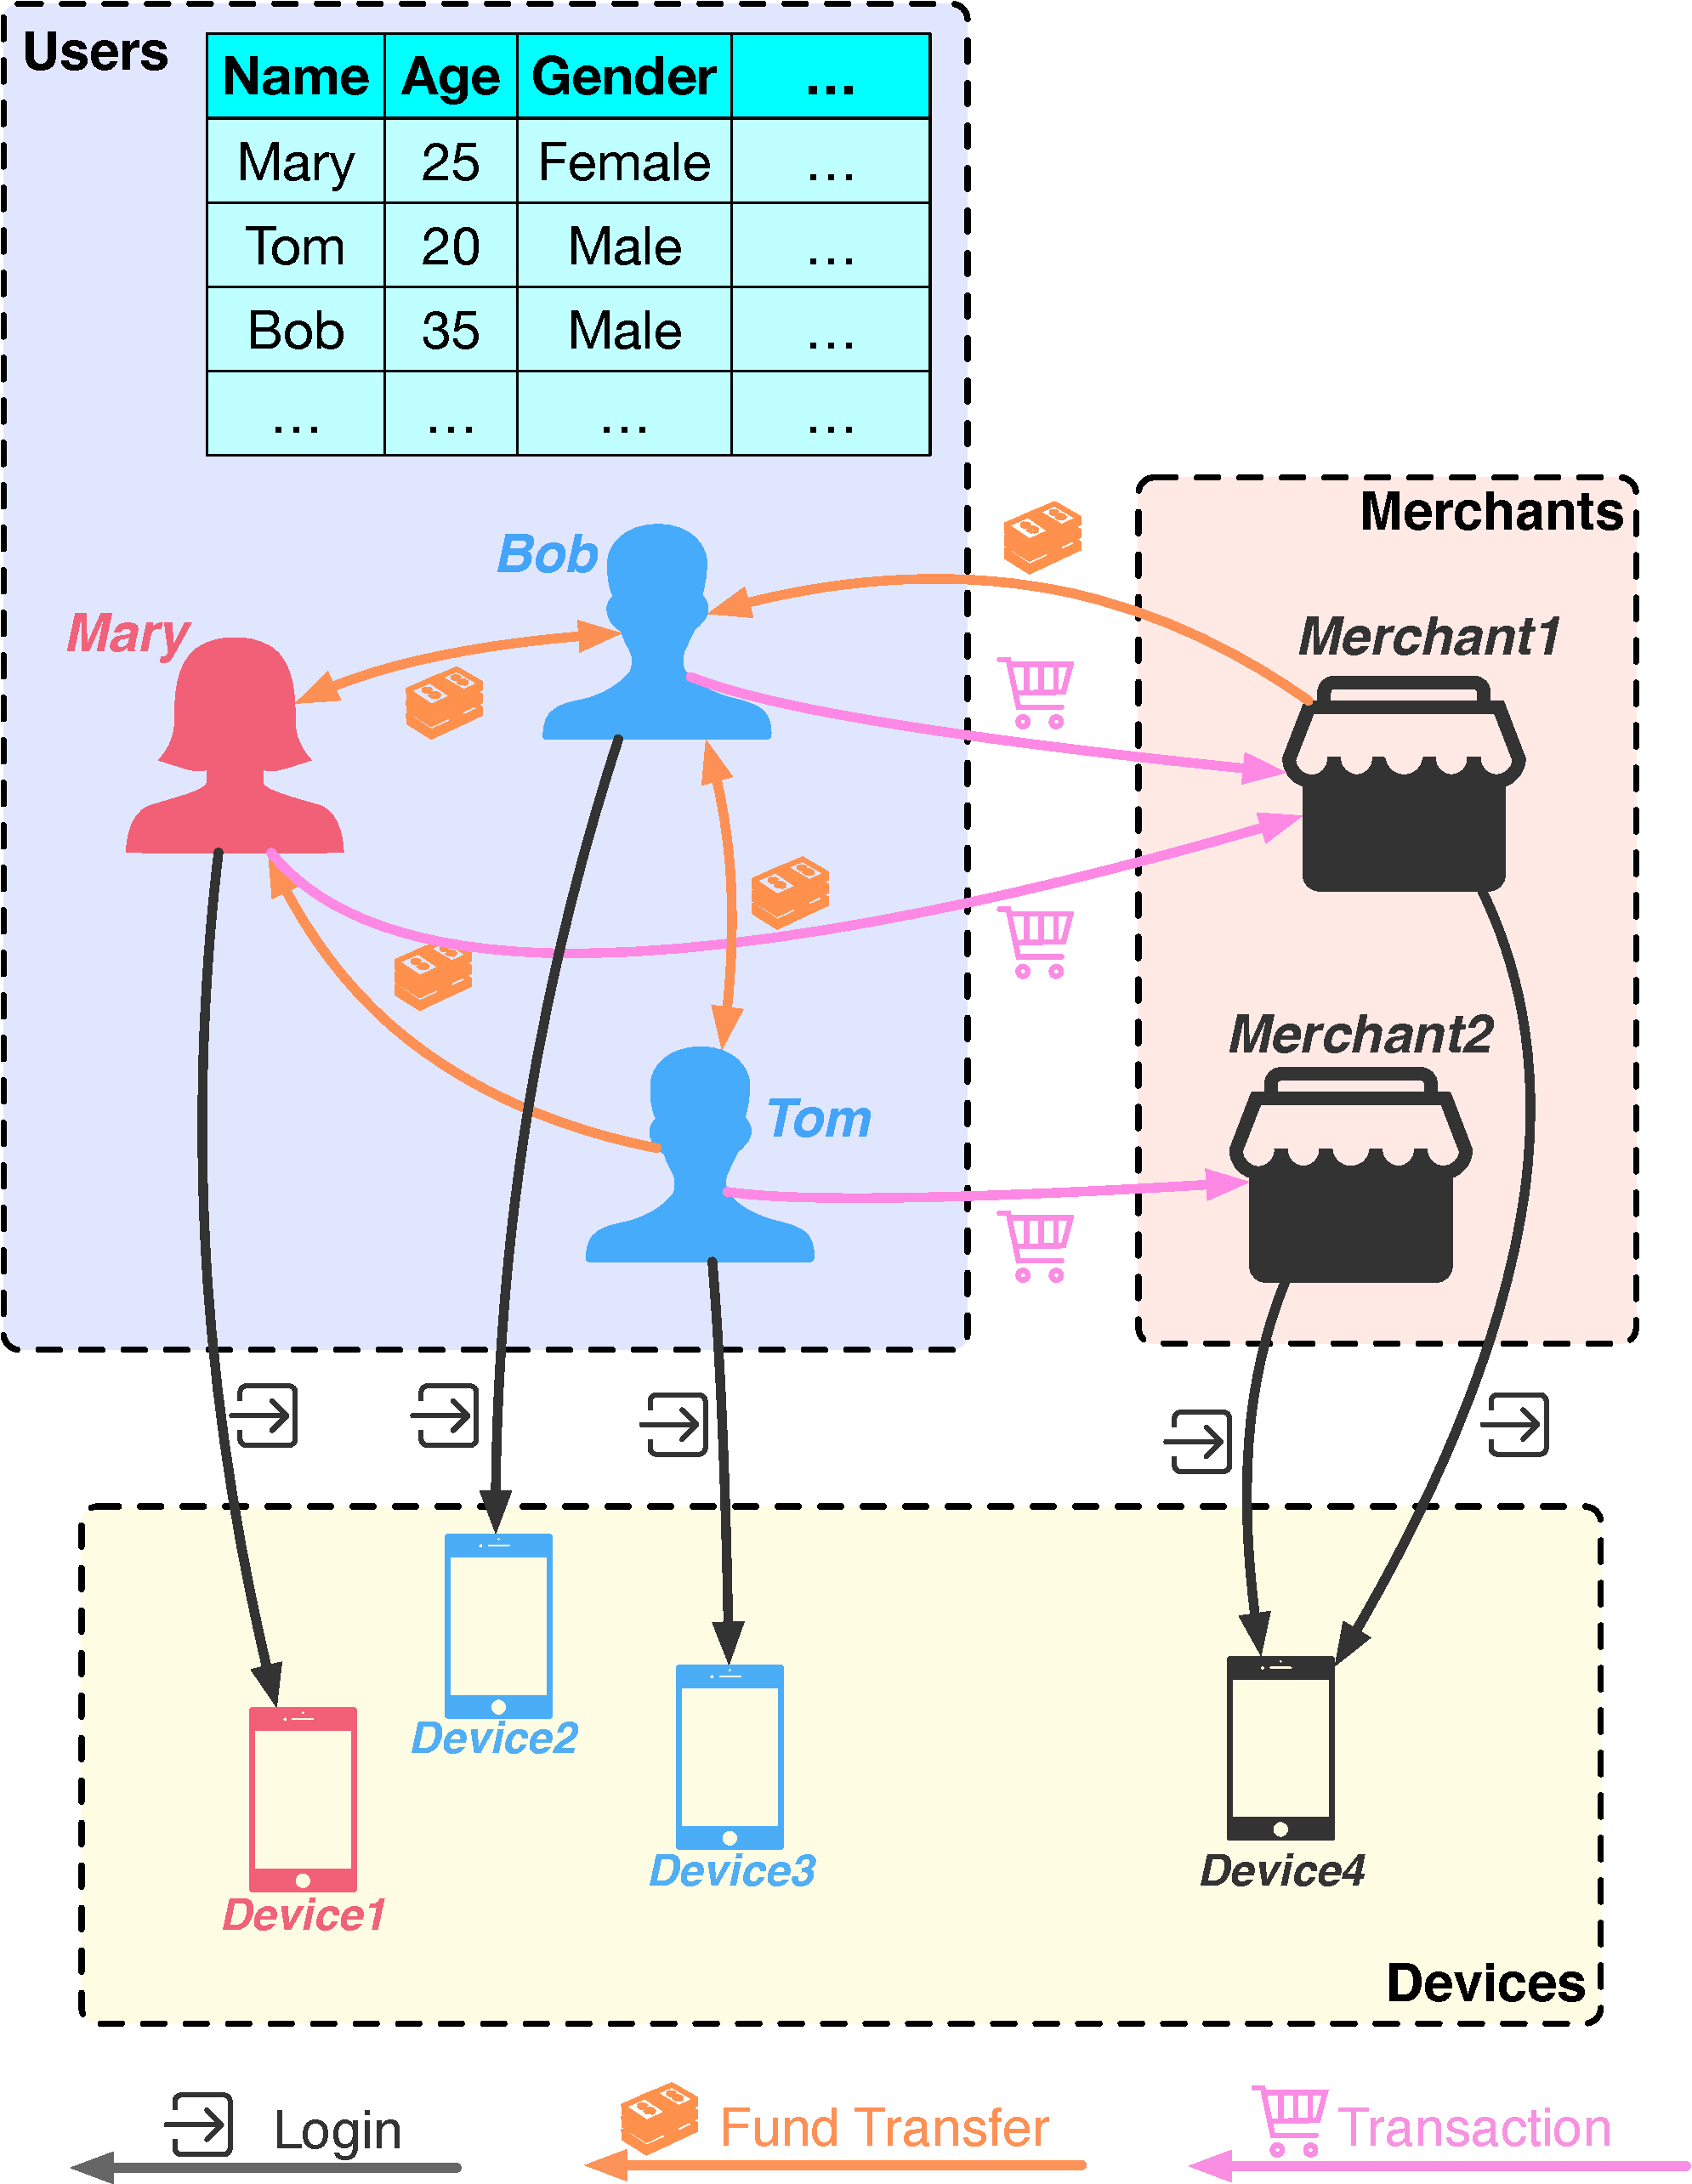
\includegraphics[width=4.5cm]{image/HIN_demo_2.pdf}\label{fig-hin}}
\subfigure[Network schema and meta-path examples]{
  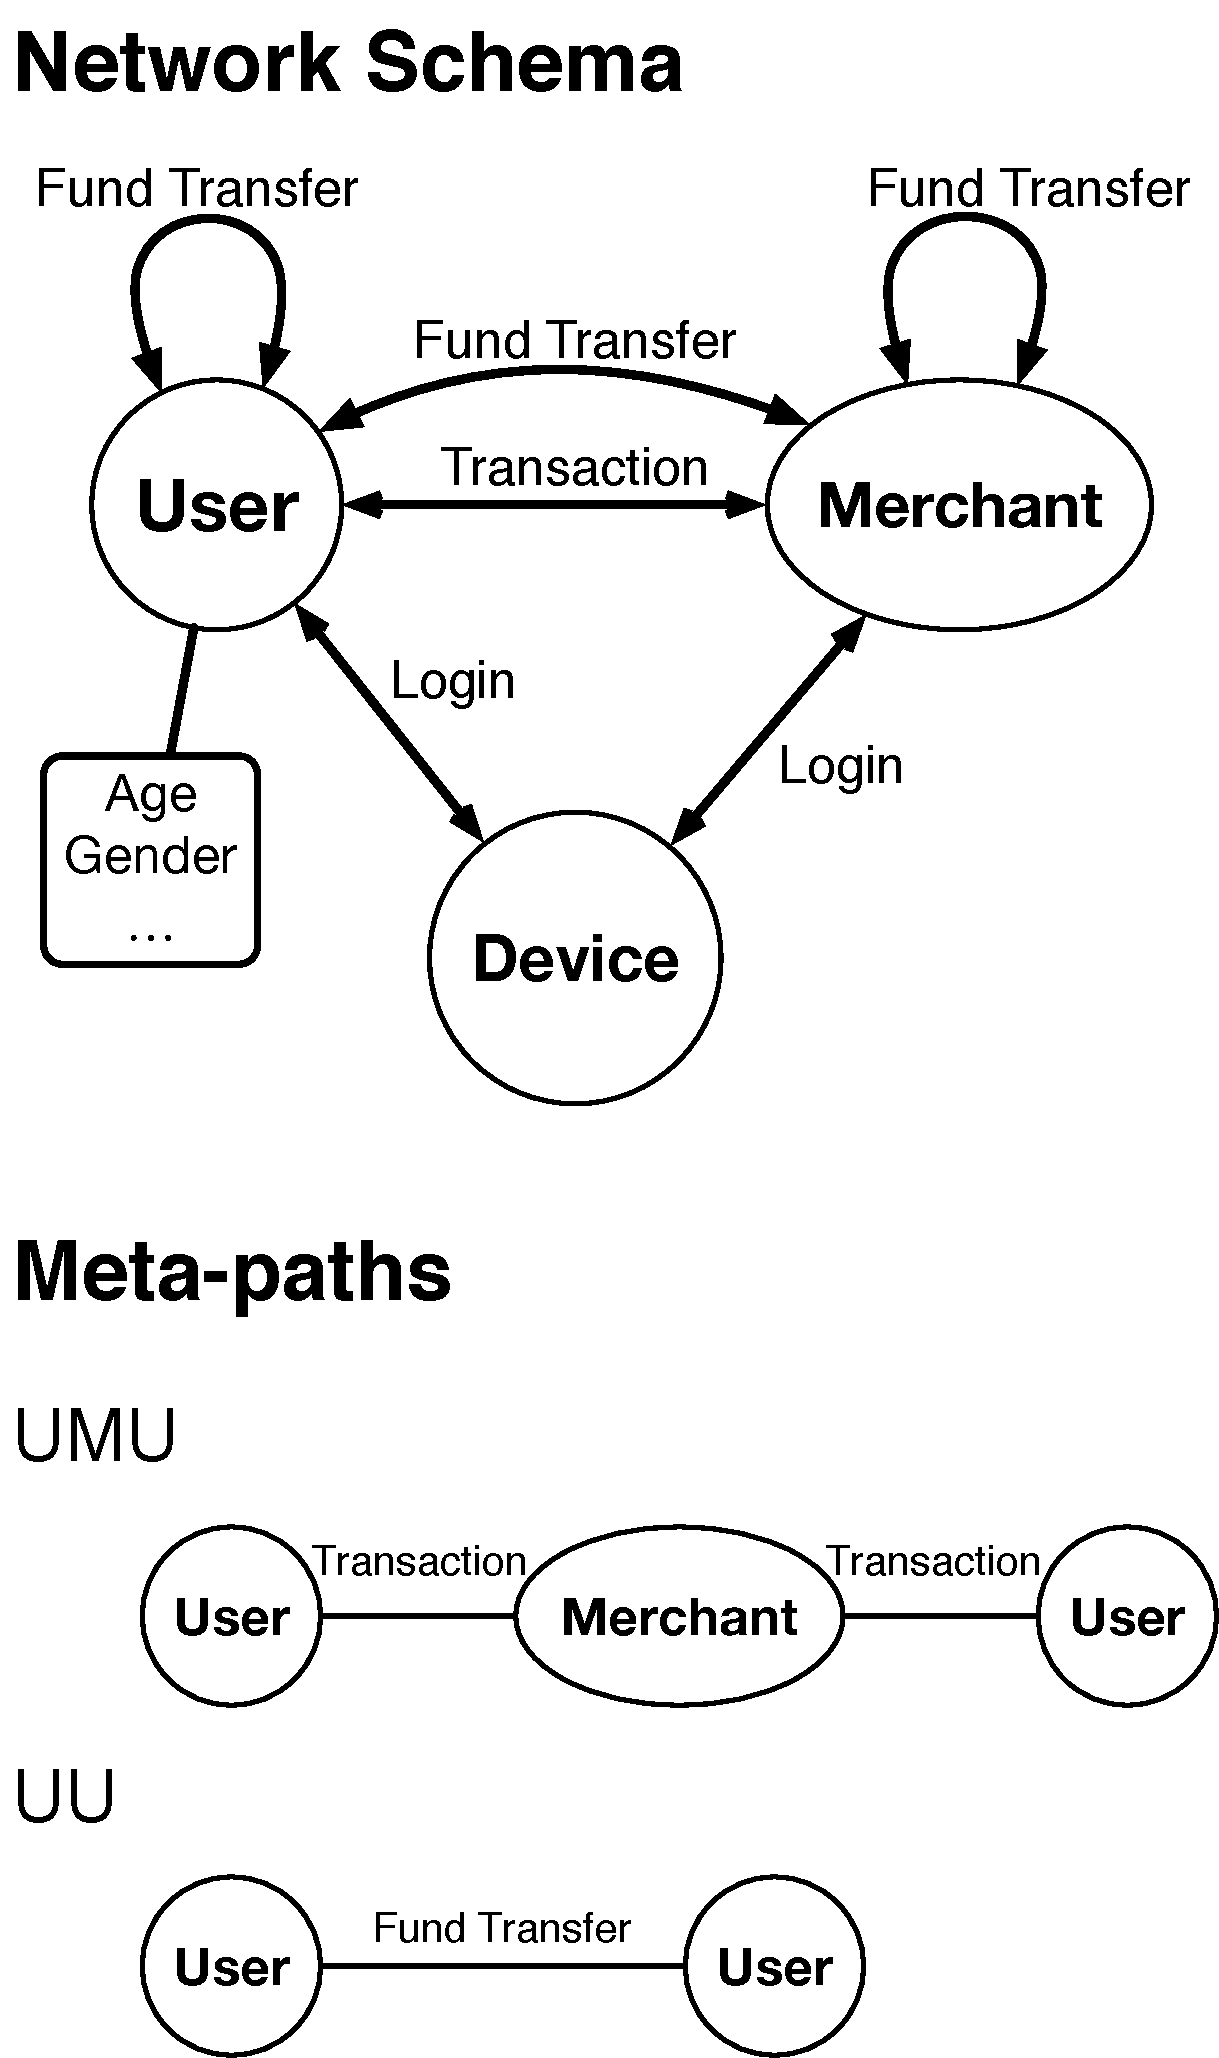
\includegraphics[width=3.5cm]{image/HIN_schema.pdf}\label{fig-hin_schema}}
\caption{The AHIN of the scenario of credit payment service.}
\label{fig:network_analysis}
\end{figure}


In fact, there are rich interaction relations in the scenario of credit payment service, which are really important to the cash-out user detection problem.  
Fig. \ref{fig-hin} demonstrates a general scenario of credit payment service, where there are three types of objects: users, merchants, and devices (the way to access services, e.g., websites, desktops, mobile apps, wifi devices, etc.). 
Besides the attribute information, these objects also have rich interaction information \eg the fund transfer relation among users, the login relation between users and devices, and the transaction relation between users and merchants. 
The cash-out users not only have abnormal features, but also behavior abnormally in interaction relations. 
For example, the cash-out users may simultaneously have many transaction and fund transfer interactions with particular merchants, which is hard to be exploited by traditional feature extraction. 

In order to exploit the interaction relations and feature information, we propose to model the scenario of credit payment service with an \emph{\textbf{A}ttributed \textbf{H}eterogeneous \textbf{I}nformation \textbf{N}etwork} (AHIN). 
The recently emerging \emph{\textbf{H}eterogeneous \textbf{I}nformation \textbf{N}etwork} (HIN)~\citep{shi2017survey}, consisting of multiple types of nodes and links, has been proposed as a powerful information modeling method for characterizing data heterogeneity~\citep{sun2011pathsim,zhao2017meta}. 
Furthermore, in order to incorporate the attribute information of objects, we extend traditional HIN to AHIN, where objects in HIN may contain attributes (or termed as features). 
Fig.~\ref{fig-hin_schema} shows the network schema of the AHIN in the scenario of credit payment service, which clearly illustrates the objects and their interactions. 
Several efforts have been made for mining HIN and shown promising performance in various kinds of applications~\citep{dong2017metapath2vec,sun2012mining,shi2018heterogeneous}.
However, they are usually designed for specific task and only exploit structure information, so they cannot be directly applied for the AHIN and the cash-out user detection problem. 

In this paper, we first study the cash-out detection problem under the AHIN framework, and propose a novel \textbf{H}ierarchical \textbf{A}ttention mechanism based \textbf{C}ash-out \textbf{U}ser \textbf{D}etection model, called HACUD. The basic idea of HACUD is to significantly enhance the feature representation of objects through fully exploiting interaction relations, i.e., with the help of meta-path based neighbors in AHIN. Inspired by~\citep{Kipf2016Semi,zhang2018anrl} and our observations on real data, we assume that the feature representation of objects, besides intrinsic features, are also constituted by the features of their neighbors. We propose the concept of meta-path based neighbors to exploit rich structure information in AHIN. That is, we can find neighbors of a node through the assigned meta-path (a relation sequence connecting two nodes). It has several advantages: (1) It can capture different aspects of structure information through different meta-paths~\citep{han2018aspect}; (2) It greatly reduces the dimension of representation space, compared to traditional network representation learning methods; (3) It is potential to predict new-coming nodes dynamically. Furthermore, we assume that object attributes and meta-paths have different importances, and elaborately design a hierarchical attention mechanism to learn user preferences towards attributes and meta-paths. Specifically,  the first layer of our attention mechanism models the user's attention in the feature space (\ie attributes), while the second layer captures the different contributions of different meta-paths for the prediction task. Finally, a cash-out probability is predicted based on aggregated feature representation with a multi-layer perceptron. 

In summary, our work has the following contributions. 

\textbullet \  We are the first to study the cash-out users detection problem, which is a very important and widely existing problem in financial fraud field. 

\textbullet \  We propose to model the cash-out user detection problem as a classification problem in AHIN which is constituted by different types of objects and their rich interactions in the scenario
of credit payment service.

\textbullet \  We propose a novel model HACUD to solve the problem, which employs meta-path based neighbors to fully exploit structure information and a hierarchical attention mechanism to automatically learn the importance of attributes and meta-paths. 

\textbullet \  Extensive experiments on two real datasets illustrate the best performance of the proposed HACUD compared to the state of arts, as well as the benefits of hierarchical attention mechanism.
%in cash-out user detection problem shows that our proposal outperforms several state-of-the-art methods.
      

%\input{sec-data}
\section{Preliminary}
A HIN is a special kind of information network, which contains either multiple types of objects or multiple types of links~\citep{sun2012mining}. In order to integrate widely existing attribute information of objects, we further extend HIN to attributed heterogeneous information network (AHIN) as follows.
\begin{myDef}
\textbf{Attributed Heterogeneous Information Network} (AHIN). An AHIN is denoted as $\mathcal{G} = \{\mathcal{V}, \mathcal{E}, \mathbf{X}\}$ consisting of an object set $\mathcal{V}$, a link set $\mathcal{E}$ and an attribute information matrix\footnote{ In our work, we discretize the original attributes to the same dimension. } $\mathbf{X} \in \mathbb{R}^{|\mathcal{V}| \times k}$. An AHIN is also associated with a node type mapping function $\phi: \mathcal{V} \rightarrow \mathcal{A}$ and a link type mapping function $\psi: \mathcal{E} \rightarrow \mathcal{R}$. $\mathcal{A}$ and $\mathcal{R}$ denote the sets of predefined object and link types, where $|\mathcal{A}| + |\mathcal{R}| > 2$.
\end{myDef}

In AHINs, two objects can be connected via different semantic paths, which are called meta-paths.
\begin{myDef}
\textbf{Meta-path}~\citep{sun2011pathsim}. A meta-path $\rho$ is defined as a path in the form of $A_1 \xrightarrow{R_1} A_2 \xrightarrow{R_2} \cdots \xrightarrow{R_l} A_{l+1}$ (abbreviated as $A_1A_2 \cdots A_{l+1}$), which describes a composite relation $R = R_1 \circ R_2 \circ \cdots \circ R_l$ between object $A_1$ and $A_{l+1}$, where $\circ$ denotes the composition operator on relations.
\end{myDef}

\begin{exmp}
As shown in Fig.~\ref{fig-hin}, we construct an AHIN to model the scenario of credit payment service in which cash-out fraud usually happens. It consists of multiple types of objects(\ie User ($U$), Merchant ($M$), Device ($D$)) with rich attributes and relations (\ie fund transfer relation between users and transaction relation between users and merchants). In the AHIN, two users can be connected via multiple meta-paths, \eg ``User-\scriptsize (fund transfer) \normalsize-User'' ($UU$) and ``User-\scriptsize (transaction) \normalsize-Merchant-\scriptsize (transaction)\normalsize -User" ($UMU$). Different meta-path always convey different semantics. For example, the $UU$ path connects users having fund transfer from one to another, while the $UMU$ connects users having transactions with the same merchants. 
\end{exmp}

As a major technical approach, meta-path based data mining methods have been extensively studied in HINs~\citep{shi2017survey}. Giving a meta-path $\rho$, there exists multiple specific neighbors \wrt each user. This neighbors set can reveal semantics and structure information of users in AHIN. 
\begin{myDef}
\textbf{Meta-path based Neighbors}. Giving a user $u$ in an AHIN, the meta-path based neighbors is defined as the set of aggregate neighbors under the given meta-path for the user $u$ in the AHIN.
\end{myDef}

\begin{exmp}
Take Fig.~\ref{fig-hin} as an example. Giving the meta-path $UU$, the neighbors of ``Mary" are ``Bob" and ``Tom". Similarly, the neighbors of "Mary" based on meta-path UMU are ``Tom''. Obviously, meta-path based neighbors can exploit different aspects of structure information in AHIN.
\end{exmp}

Here we model the scenario of credit payment service with an AHIN which can comprehensively integrate rich features and  interaction information. Furthermore, we define the cash-out user detection problem under the AHIN framework as follows. 

\begin{myDef}
\textbf{Cash-out User Detection Problem under AHIN}. In the cash-out user detection problem, various kinds of objects and their interactions can be modeled as an AHIN $\mathcal{G} = \{\mathcal{V}, \mathcal{E}, \mathbf{X}\}$. In our setting, we focus on detecting cash-out users who are a subset of the node set, denoted as $\mathcal{U} \subset \mathcal{V}$. We assign a label $y_u \in \{0, 1\}$ on each user $u \in \mathcal{U}$ to indicate whether he/she is a cash-out user or not. Given the AHIN $\mathcal{G} = \{\mathcal{V}, \mathcal{E}, \mathbf{X}\}$ and the training set $\mathcal{D} = \{ (u, y_u) \}$, the goal is to predict the cash-out probability $p_{u^t}$ of user $u^t$ in the test set. %Note that the user $u^t$ may never appear in the training set $\mathcal{D}$.
\end{myDef}

\begin{figure}
  \centering
  % Requires \usepackage{graphicx}
  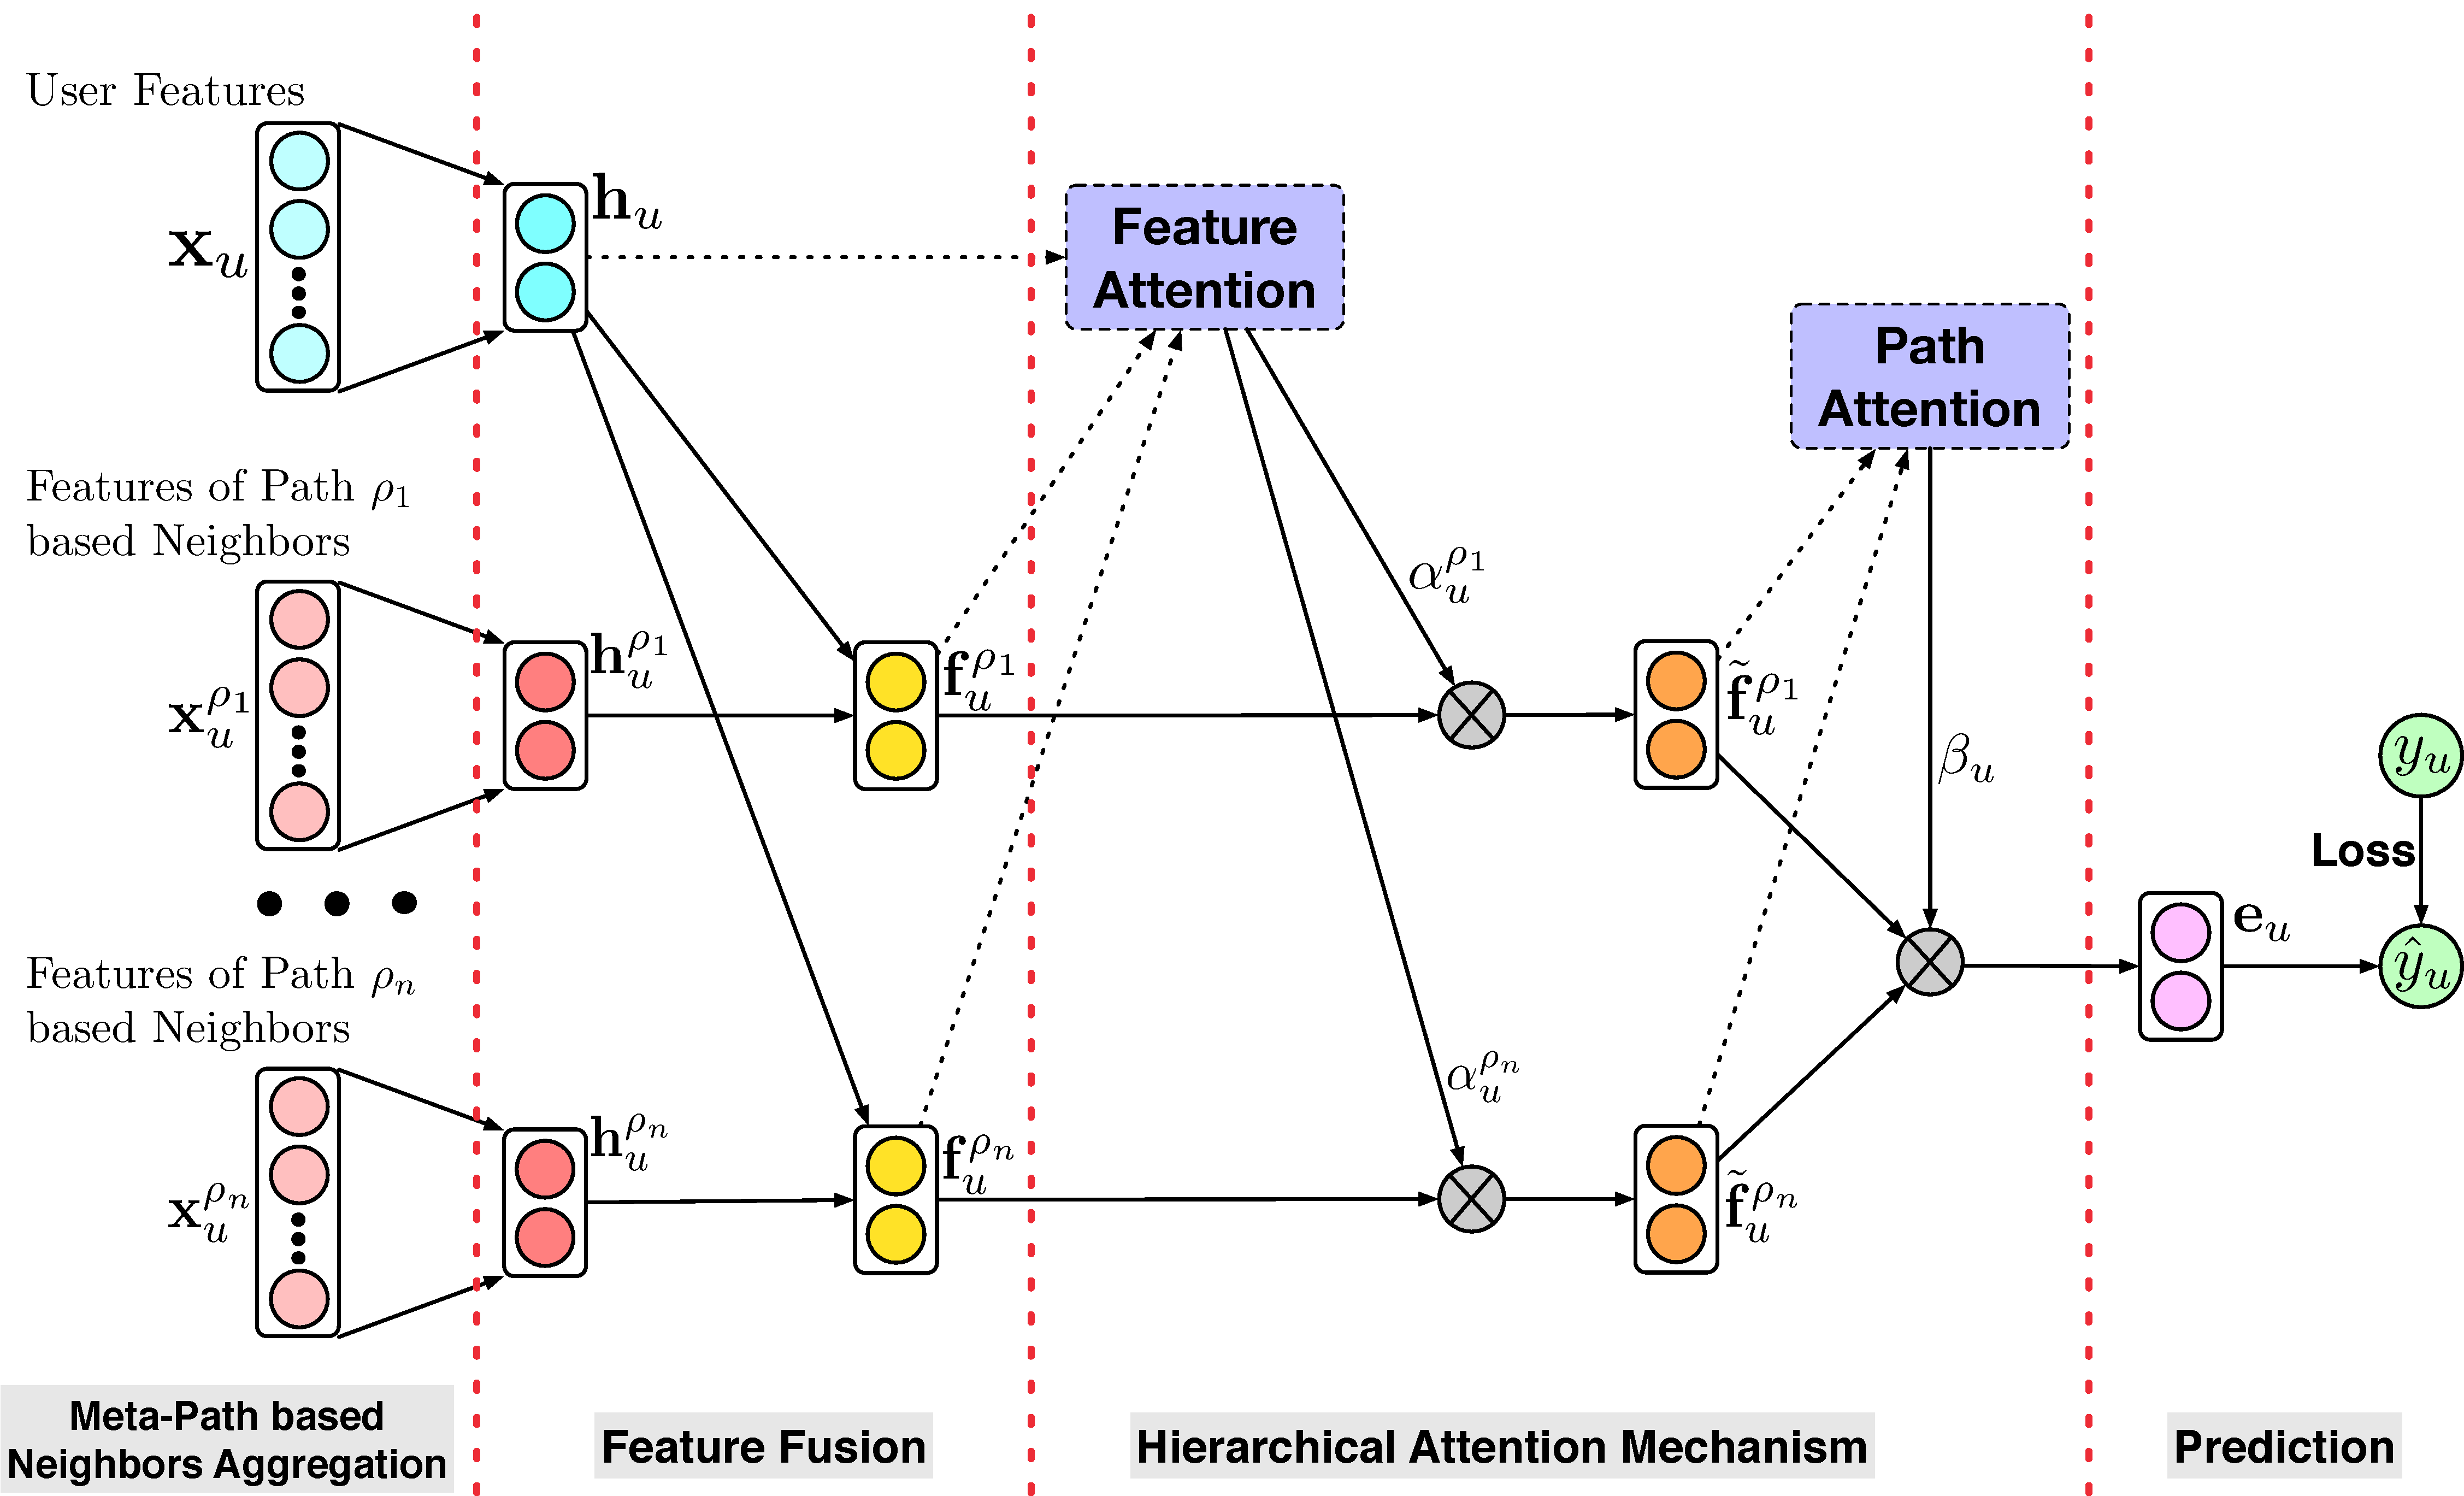
\includegraphics[width=8.5cm]{image/Model_Attention.pdf}\\
  \caption{The architecture of the proposed model}\label{fig-model}
\end{figure}

\section{The Proposed Model}
In this section, we firstly analyze the effect of meta-path based neighbors on the cash-out user detection on real data and then present the proposed \emph{\textbf{H}ierarchical \textbf{A}ttention mechanism based \textbf{C}ash-out \textbf{U}ser \textbf{D}etection model}, called \textbf{HACUD} shortly.
We show the overall architecture of the proposed model in Fig.~\ref{fig-model}. Firstly, we aggregate neighbors for each user based on different meta-paths to integrate multiple aspects of structure information in AHIN, and then we transform and fuse the original features for better representation learning. Considering that different features and meta-paths have different importances, we design a hierarchical attention mechanism to model user preferences towards features and meta-paths. %Due to the integration of meta-path and attribute based information in AHIN, our model is expected to yield a better performance in cash-out user detection problem.

\begin{figure}[t]
\centering
\subfigure[UMU]{
  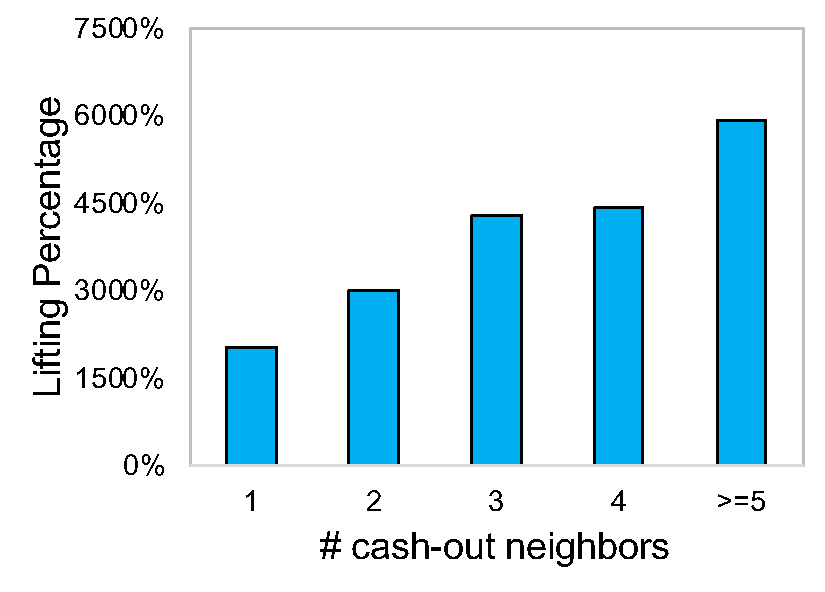
\includegraphics[width=4.0cm]{image/network_analysis_1.pdf}\label{fig:network1}}
\subfigure[UU]{
  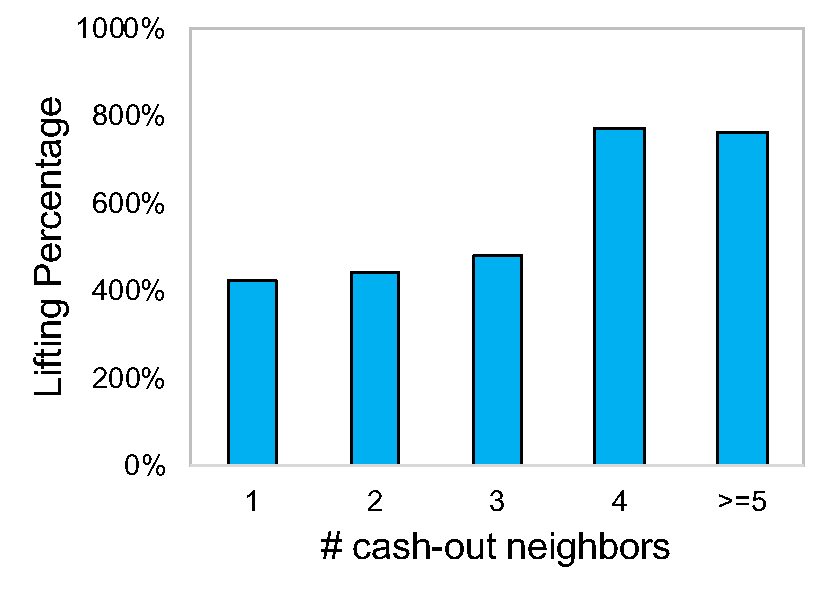
\includegraphics[width=4.0cm]{image/network_analysis_3.pdf}\label{fig:network3}}
%\subfigure[UMDMU]{
%  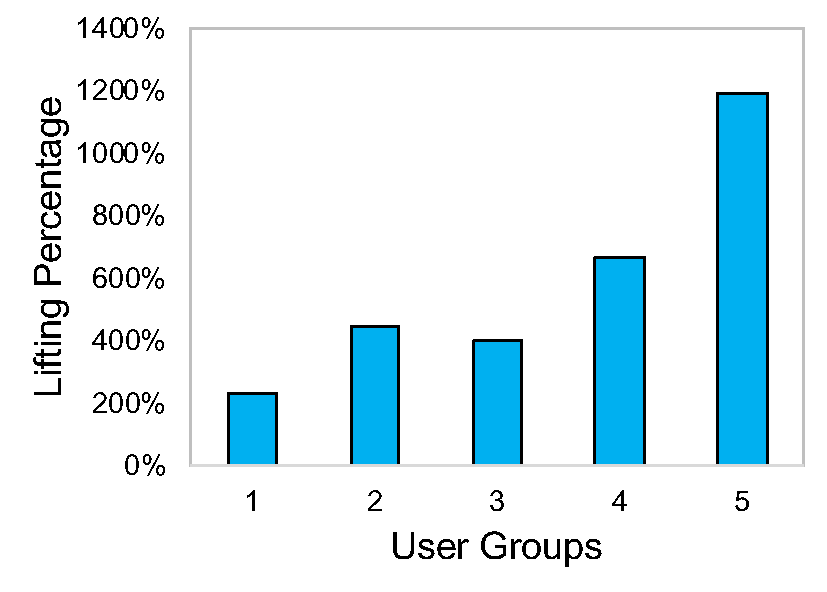
\includegraphics[width=5.6cm]{image/network_analysis_2.pdf}\label{fig:network2}}
\caption{The lifting percentages of cash-out rate in users with different amount of cash-out neighbors against users without any cash-out neighbor in two meta-paths.}%To be noted that the above results are calculated based on the real world dataset from Ant Credit Pay, an online credit payment service provided by Ant Financial Services Group.}
\label{fig:network_analysis}
\end{figure}

\subsection{Observations in Real Data}
Intuitively, the cash-out users tend to aggregate closely through different kinds of interactions.
Taking the AHIN in Fig. \ref{fig-hin} as an example, cash-out users tend to make more transactions with merchants which sell particular goods (e.g., pre-pard cards) or interact with more deceivers. 
In order to validate the aggregation of cash-out users with respect to different relations, we do experiments on the real dataset in Ant Credit Pay of Ant Financial Services Group (see Ten Days Dataset in Experiments). 

We first collect the meta-path based neighbors of each user based on two meta-paths ($UMU$ meaning users having transactions with the same merchants and $UU$ meaning users having fund transfer from one to another). 
For each meta-path, we count the number of neighbors who are cash-out user (called cash-out neighbor), and divide all users into different groups with respect to the number of their cash-out neighbors.
The cash-out rate (i.e., the proportion of cash-out users) is calculated in each group. The lifting percentages of cash-out rate in different user groups against users without any cash-out neighbor, with respect to two meta-paths, are presented in Fig. \ref{fig:network_analysis}. 
We have the following observations.

(1) Users with higher cash-out rate tend to have more cash-out neighbors.
This observation illustrates that 
%meta-path neighbors have great impact on recognizing cash-out users and can be utilized  to enhance the target users' representations. 
meta-path based neighbors have consistent behaviors with the original user, which implies that the features of users can stem from that of their meta-path based neighbors.

(2) Different meta-path based neighbors have different impacts on users. In Fig. \ref{fig:network_analysis}, two meta-paths yield different lifting percentages. %especially for users with no less than 5 cash-out neighbors through UMU path, the cash-out rate is around 60 times larger than users without any cash-out neighbor (Fig \ref{fig:network1}). 
%It inspires us to model this problem with a hierarchical attention mechanism, which automatically learns the importance of attributes and meta-paths.
It inspires us that different meta-paths have different importances on users, which can be captured by recent emerging attention mechanism.

\subsection{Meta-path based Neighbors Aggregation}
Inspired by recently emerging graph convolutional networks~\citep{Kipf2016Semi,dai2016discriminative} and the above observations on real data, we think that feature representations of objects, besides their intrinsic features, are also composed of the features of their neighbors. Based on this idea, we aggregate meta-path based neighbors for each user. 
%To capture multiple aspect of information in AHIN, we collect neighbors based on different meta-paths. For each user $b$, we denote the neighborhood based on a meta-path $\rho$ as $\mathcal{N}^{\rho}_u$. In order to adapt our model to large scale network, inspired by the recent progress on 
Specifically, similar to recent attributed network embedding~\citep{liang2018semi,zhang2018anrl}, we adopt to represent a node \wrt a certain meta-path via aggregating features of its neighbors rather than the one-hot representation of its neighbors. For each user $u$, we can obtain the \emph{aggregated features based on meta-path} $\rho$ as below:
\begin{equation}
\mathbf{x}^{\rho}_u = \sum_{j \in \mathcal{N}^{\rho}_u}{w^{\rho}_{uj} * \mathbf{x}_j},
\end{equation}
where $\mathcal{N}^{\rho}_u$ is the neighbors of node $j$ based on meta-path $\rho$ and $\mathbf{x}_j$ represents the attribute information vector associated with node $j$. The given link weight $w_{uj} > 0$ for weighted networks and $w_{uj} = 1$ for unweighted networks.


\subsection{Feature Fusion}
For each user $u$, we can obtain its own feature $\mathbf{x}_u$ as well as a set of its neighbor aggregation features based on multiple meta-paths $\{\mathbf{x}^{\rho}_u\}_{\rho \in \mathcal{P}}$ where $\mathcal{P}$ denotes the set of meta-paths. For better representation learning, we set up a \emph{feature fusion} part to  transform and fuse the original features. 

Firstly, we project the original sparse features to the low-dimensional dense representations, and obtain the \emph{latent representations} of user $u$ and his/her neighbors based on different meta-paths (i.e., $\mathbf{h}_u$ and $\mathbf{h}_u^\rho$), respectively: %which can be formulated as follows:
%\begin{eqnarray}
%\mathbf{h}_u &=& \mathbf{W}\mathbf{x}_u + \mathbf{b}, \\
%\mathbf{h}^{\rho}_u &=& \mathbf{W}^{\rho}\mathbf{x}^{\rho}_u + \mathbf{b}^{\rho}, %\nonumber
%\end{eqnarray}
\begin{equation}
\mathbf{h}_u = \mathbf{W}\mathbf{x}_u + \mathbf{b}, \ \ \ \ \mathbf{h}^{\rho}_u = \mathbf{W}^{\rho}\mathbf{x}^{\rho}_u + \mathbf{b}^{\rho},
\end{equation}
where $\mathbf{W}^* \in \mathbb{R}^{D \times d}$ and $\mathbf{b}^* \in \mathbb{R}^{d}$ are the weight matrix and bias vector, respectively. $D$ is the dimension of original feature space\footnote{The original attributes are discretized to sparse  $D$-dimensional feature as the model input} and $d$ is the dimension of latent representations. Next, we fuse the latent representations of a user and his/her neighbors based on each meta-path and add a fully-connected layer for more complicated interaction. For a meta-path $\rho$, we formulate the above procedure and obtain the \emph{fusional representation} $\mathbf{f}_u^{\rho}$ \wrt meta-path $\rho$ as below,
\begin{equation}
\mathbf{f}^{\rho}_u =\text{ReLU}(\mathbf{W}_{F}^{\rho}g(\mathbf{h}_u, \mathbf{h}^{\rho}_u) + \mathbf{b}^{\rho}_F).
\end{equation}
Here, $\textbf{W}_F^{\rho} \in \mathbb{R}^{d \times 2d}$ and $\mathbf{b}^{\rho}_F \in \mathbb{R}^{d}$ represent the weight matrix and bias vector based on meta-path $\rho$, respectively. $g(\cdot , \cdot)$ is the fusion function, which can be concatenation, addition or element-wise product (In our implementation, $g(\cdot , \cdot)$ is concatenation).
\subsection{Hierarchical Attention}
Intuitively, different users are likely to have different preferences over the features based on different meta-paths as well as attribute information. Concretely, a user may place different importances to different-aspect features based on meta-paths. Moreover, features also have different importances for the prediction task.
%the various aspects based on different meta-paths, and an important aspect sometimes can highly contribute to the prediction for the high risk users. Furthermore, different meta-path can also contribute to the prediction unequally since they convey different semantics. 
Due to the effectiveness of attention mechanism in various machine learning tasks~\citep{hu2018leveraging,Cheng2018A,you2016image}, we design a hierarchical attention mechanism to capture user preferences towards features and meta-paths.
\subsubsection{Feature Attention}
Since different features might not contribute to the prediction task equally, we learn the aspect-specific attention weights over features conditioned on the involved user based on each meta-path. Given the user latent representation $\mathbf{h}_u$ and latent representation of his/her neighbors $\mathbf{f}^{\rho}_u$ based on meta-path $\rho$ , we adopt a two-layer neural network to implement the attention.
%\begin{equation}
%\bm{\alpha}_b^{\rho} = \text{RELU}(\mathbf{W}_f^2\text{RELU}(\mathbf{W}_f^1[\mathbf{h}_b ; \mathbf{f}_b^{\rho}] +\mathbf{b}_f^1) + \mathbf{b}_f^2),
%\end{equation}
\begin{eqnarray}
\bm{v}_u^{\rho} &=& \text{ReLU}(\mathbf{W}_f^1[\mathbf{h}_u ; \mathbf{f}_u^{\rho}] +\mathbf{b}_f^1), \\
\bm{\alpha}_u^{\rho} &=& \text{ReLU}(\mathbf{W}_f^2\bm{v}_u^{\rho} + \mathbf{b}_f^2),
\end{eqnarray}
where $\mathbf{W}_f^*$ and $\mathbf{b}_f^*$ denote the weight matrix and bias vector, respectively and $[\cdot ; \cdot]$ represents the concatenation of two vectors. Following the standard setting of neural attention networks, we normalize the above attention scores with the softmax function to obtain the final attention weights.
\begin{equation}
\hat{\alpha}_{u, i}^{\rho} = \frac{\exp(\alpha_{u, i}^{\rho})}{\sum_{j = 1}^{K}{\exp(\alpha_{u, j}^{\rho})}}.
\end{equation}
Then, the final representation of user $u$ \wrt a meta-path $\rho$ can be computed as follows,
\begin{equation}
\label{equ-f-tilde}
\widetilde{\mathbf{f}}^{\rho}_u = \bm{\hat{\alpha}}_u^{\rho} \bigodot \mathbf{f}_u^{\rho},
\end{equation}
where ``$\bigodot$'' denotes the element-wise product.
\subsubsection{Path Attention}
Given a user, following the above steps, we could obtain multiple representations based on multiple meta-paths, which are expected to collaborate with each other for better prediction. Following~\citep{qu2017attention}, we learn  the attention weights over different meta-paths for collaboration. Specifically, we define the attention weight of meta-path $\rho$ for user $u$ using a softmax unit as follows:
\begin{equation}
\beta_{u, \rho} = \frac{\exp({\mathbf{z}^{\rho}}^{\mathrm{T}} \cdot \mathbf{\widetilde{f}}^C_u)}{\sum_{\rho' \in \mathcal{P}}{\exp({\mathbf{z}^{\rho^\prime}}^{\mathrm{T}} \cdot \mathbf{\widetilde{f}}^C_u)}},
\end{equation}
where $\mathbf{z}^{\rho} \in \mathbb{R}^{|\mathcal{P}| * d}$ is the attention vector for meta-path $\rho$ and $\widetilde{\mathbf{f}}^C_u$ is the concatenation of user $u$'s representations \wrt all meta-paths ($\ie$ $\widetilde{\mathbf{f}}^{\rho}_u$). After obtaining the path attention scores $\beta_{u, \rho}$, the final representation aggregating all meta-paths is given as the following weighted sum form:
\begin{equation}
\mathbf{e}_u = \sum_{\rho \in \mathcal{P}}{\beta_{u, \rho} * \mathbf{\widetilde{f}}^{\rho}_u},
\end{equation}
where $\mathbf{\widetilde{f}}^{\rho}_u$ is the representation of neighbors for user $u$ based on meta-path $\rho$ in Eq.~\ref{equ-f-tilde}.

\subsection{Model Learning}
Since neural networks have shown strong ability in modeling the complex interactions~\citep{he2017neural}, we feed the obtained final representation (\ie $\mathbf{e}_u$) into multiple fully connected neural networks as follows,
\begin{equation}
\mathbf{z}_u = \text{ReLU}(\textbf{W}_{L} \cdots \text{ReLU}(\mathbf{W}_1\mathbf{e}_u + \mathbf{b}_1) + \mathbf{b}_{L}),
\end{equation}
where $\mathbf{W}_*$ and $\mathbf{b}_*$ respectively denote the weight matrix and the bias vector for each layer. The predicted cash-out probability is obtained via a regression layer with a sigmoid unit:
\begin{equation}
p_u = \text{sigmoid}(\mathbf{w}_p^{T}\mathbf{z}_u + b_p).
\end{equation}
Here $\mathbf{w}_p$ and $b_p$ are the weight vector and the bias, respectively. As our task is classification, we model the objective function with maximum likelihood estimation, which can be formulated as follows:
\begin{equation}
\label{equ-objective}
\mathcal{L}(\Theta) = \sum_{\langle u, y_u \rangle \in \mathcal{D}}(y_u\log(p_u) + (1 - y_u)\log(1 - p_u)) + \lambda ||\Theta||^2_2, 
\end{equation}
where $y_u$ and $p_u$ represent the ground truth and the predicted cash-out probability of user $u$, respectively. $\Theta$ is the parameter set of the proposed model and $\lambda$ is the regularizer parameter. The stochastic gradient descent (SGD) or its variants are adopted for optimization.

\subsection{Discussion}
As mentioned above, the proposed model is a flexible framework to leverage structure and attribute information through capturing multiple aspects in AHIN. Based on different meta-paths, we can integrate various kinds of heterogeneous information to enhance the prediction performance. Moreover, we represent a user via the feature aggregation of his/her neighbors based on meta-paths, which is a natural way to combine network structure and attribute information. Compared to traditional network embedding methods~\citep{wang2016structural,dai2016discriminative}, which represent nodes via their context (\eg adjacency matrix), our method is more suitable for large-scale networks. Specifically, the dimension of original input can be reduced from $\mathcal{O}(|\mathcal{V}|)$ to $\mathcal{O}(D)$, where $|\mathcal{V}|$ is the total number of nodes in network and $D$ is the feature dimension after  discretization for each user ($D \ll |\mathcal{V}|$). For a new user which never appears in training set, the proposed model can also learn the representation through his/her meta-path based neighbors in networks. Therefore, our model has the ability to give predictions dynamically to some extent.

\section{Experiments}
In this section, we construct the experimental evaluation and present the result analysis.

%\begin{table}[!htbp]
%\centering
%\caption{Datasets} \label{tab-data}
%\begin{tabular}{c|c|c}%
%\hline
%{Dataset} & {Time Interval} & {\#user} \\
%\hline
%\multirow{2}{*}{Ten Days} & {20180321 $\sim$ 20180331} & {1884174}\\
%\cline{2-3}
%\multirow{2}{*}{} & {20180501} & {177489}\\
%\hline
%\multirow{2}{*}{One Month} & {20180301 $\sim$ 20180331} & {5160229}\\
%\cline{2-3}
%\multirow{2}{*}{} & {20180501} & {177489}\\
%\hline
%\end{tabular}
%\end{table}

\subsection{Evaluation Dataset}
With the real-world datasets in Ant Credit Pay, an online credit payment service provided by Ant Financial Services Group,  we extract two sub-datasets for the evaluation, namely Ten Days Dataset (contains 1.88 million users ranging  from 2018/03/21 to 2018/03/31 for training) and One Month Dataset (contains 5.16 million users ranging from 2018/03/01 to 2018/03/31 for training). For both datasets, we predict the cash-out probability of users in 2018/05/01 (around 0.17 million users). In our datasets, we define the positive samples as users who have involved in suspected cash-out transactions within one month and the negative samples as users who have never involved in suspected cash-out transactions within one month. Since we utilize data in the next month when defining the label, the time interval between training and test set is one month. To be noted that since the cash-out fraud is very much in the minority among all transactions, the negative examples are sampled to keep the cash-out rate at around 2\% in our datasets.  

We construct an attributed heterogeneous information network based on the two datasets, consisting of  56.75 million users and 0.51 million merchants. In addition, the AHIN contains 77.40 million fund transfer relations between users and 20.64 million transaction relations between users and merchants. 
%consisting of multiple type of entities (\ie user (around 56.75 million) and merchant (around 507.51 thousand)) and relations (\ie fund transfer (around 77.40 million) and transaction (around 20.64 milion)) 
We extract 123 attributes for each user, including user profile, credit history, transaction summarizing, recent behaviors in other relative businesses and so on. Considering the scale of attribute value and the existence of missing value, we preproccess the two datasets with feature discretization.  

\begin{table}[t]
\footnotesize
\centering
\caption{Selected meta-paths and meta-path based neighbors statistics. } \label{tab-mp}
\begin{tabular}{c|c}%
\hline
\multirow{2}{*}{Meta-paths} & {\#Neighbors }\\%
\multirow{2}{*}{} & {(Min / Max / Avg.)} \\
\hline
{User-\scriptsize (transaction) -\small Merchant-\scriptsize (transaction)\small -User} & {1 / 16860 / 309}\\
\hline
{User-\scriptsize (fund transfer) \small-User}& {1 / 26235 / 150}\\
\hline
{User-\scriptsize (transaction) \small-Merchant} & {1 / 81 / 4} \\
\hline
\end{tabular}
\end{table}

\subsection{Evaluation Metrics}
We use the widely adopted metric to measure the performance of cash-out user detection , namely \textbf{AUC} (\ie Area Under the ROC Curve). The AUC metric is defined is:
\begin{equation}
AUC = \frac{\sum_{u \in \mathcal{U}^+}{rank_{u}} - \frac{|\mathcal{U}^+| \times (|\mathcal{U}^+| + 1)}{2}}{|\mathcal{U}^+| \times |\mathcal{U}^-| }.
\end{equation}
Here, $\mathcal{U}^+$ and $\mathcal{U}^-$ denotes the positive and negative set in the test set, respectively. And $rank_u$ indicates the rank of user $u$ via the score of prediction.


\begin{table*}[t]
\centering
\caption{Results of effectiveness experiments on two datasets \wrt the dimension of latent represantation $d$. A larger value indicates a better performance.} \label{tab-eff}
\begin{tabular}{c|c|c|c|c|c|c|c|c}%
\hline
\multirow{3}{*}{Algorithm} & \multicolumn{8}{|c}{AUC}\\
\cline{2-9}
\multirow{3}{*}{} & \multicolumn{4}{|c}{Ten Days Dataset} & \multicolumn{4}{|c}{One Month Dataset}\\
\cline{2-9}
\multirow{3}{*}{} & {$d = 16$} & {$d = 32$} & {$d = 64$} & {$d = 128$} & {$d = 16$} & {$d = 32$} & {$d = 64$} & {$d = 128$}\\
\hline
Node2vec & 0.5893  &0.5913 & 0.5926 & 0.5930 & 0.5980 & 0.6063 & 0.6009 & 0.6021\\
%\hline
Metapath2vec & 0.5914 & 0.5903 & 0.5917 & 0.5920 & 0.6005& 0.5976 &  0.5995 & 0.5983\\
%\hline
{Node2vec + Feature}  & 0.6455 & 0.6464  & 0.6510 & 0.6447 & 0.6541 & 0.6561 & 0.6607 & 0.6518\\
%\hline
{Metapath2vec + Feature}  & 0.6456 &  0.6429 & 0.6469 & 0.6485 & 0.6550 & 0.6552& 0.6523 & 0.6545\\
%\hline
Structure2vec & 0.6537 & 0.6556 & 0.6598 & 0.6545 & 0.6641 &0.6632 & 0.6657 & 0.6678\\
%\hline
GBDT & 0.6389 & 0.6389 & 0.6389 & 0.6389 & 0.6467 & 0.6467 & 0.6467 & 0.6467\\

GBDT$_{Struct}$& 0.6948 & 0.6948 & 0.6948 & 0.6948 & 0.6968 & 0.6968 & 0.6968 & 0.6968\\

HACUD & \textbf{0.7066} & \textbf{0.7115} & \textbf{0.7056}& \textbf{0.7049} &\textbf{0.7132} & \textbf{0.7160} & \textbf{0.7109}&\textbf{0.7154}\\
\hline
\end{tabular}
\end{table*}

\subsection{Methods to Compare}
We consider several representative methods for the cash-out user detection task,
%The selected baselines have a comprehensive coverage of existing methods for our scene, 
%We consider two kinds of representative recommendation methods
which  can roughly be categorized into three type: (1) Attribute only or Structure only (GBDT, Node2vec, Metapath2vec). (2) Structure + Attribute (Node2vec + Feature, Metapath2vec + Feature). (3) Structure + Attribute + Label (Structure2vec, GBDT$_{Struct}$).


\textbullet \textbf{Node2vec}~\citep{grover2016node2vec} : It is a representation learning method on homogeneous network. We employ it to learn representations for nodes, ignoring node heterogeneity, and feed them into a classification model.

\textbullet \textbf{Metapath2vec}~\citep{dong2017metapath2vec} : It is a heterogeneous information network embedding method for learning node embedding with meta-path guided random walks. Similarly, we also feed the node representations into a classification model.

\textbullet \textbf{Node2vec + Feature} : We feed the features of node as well as the embeddings learned by Node2vec into a classification model.

\textbullet \textbf{Metapath2vec + Feature} : We feed the features of node as well as the embeddings learned by Metapath2vec into a classification model.

\textbullet \textbf{Structure2vec}~\citep{dai2016discriminative} : It is an effective approach for network embedding based on network structure and feature information with labeled data.

\textbullet \textbf{GBDT}~\citep{friedman2001greedy} : It is a scalable tree-based model for feature learning and classification task. We feed node feature  into GBDT.

\textbullet \textbf{GBDT$_{Struct}$} : Besides node feature, we also feed the aggregate features of meta-path based neighbors into GBDT.

\subsection{Implementation Details}
We implement the proposed model based on Tensorflow~\citep{abadi2016tensorflow}.  We utilize two hidden layers for prediction. We randomly initialize the model parameters with a xavier initializer~\citep{glorot2010understanding} and choose RMSProp~\citep{tieleman2012lecture} as the optimizer. Moreover, we set the batch size to 256, the learning rate to 0.002 and set the regularizer parameter $\lambda = 0.01$ to prevent overfitting. We report the selected meta-paths and meta-path based neighbors statistics information in Table~\ref{tab-mp}. For the other comparison methods, we optimize their parameters according to literatures. Moreover, for all baselines, we implement them on parameter server based distributed learning systems\citep{zhou2017kunpeng} for scaling up to large-scale datasets. And we select GBDT as the final classification model for the baselines.


\subsection{Experimental Results}
\paratitle{Performance Comparison}. We report the comparison results of the proposed approach and baselines \wrt the dimension of latent representation $d$ in Table~\ref{tab-eff}. The major findings from the experimental results can be summarized as follows:

(1) Our model outperforms all the baselines, which indicates that our model adopts a more principled way to leverage interaction relations and attribute information for improving prediction performance. Our model achieves the best performance where the dimension of latent representation $d = 32$. And overall, the performance change trend is smooth, indicating that our model is not very sensitive to this parameter.

(2) Among these baselines, we can find that the overall performance order is as follows: (label + attribute + structure) based methods (\ie GBDT$_{Struct}$, Structure2vec) $>$ (attribute + structure) based methods (\ie Node2vec + Feature, Metapath2vec + Feature) $>$ structure or attribute only based method (\ie Node2vec, Metapath2vec, GBDT). 
It indicates that the better performances can be achieved through fusing more information. In addition, structure information (\ie interaction relations) is really helpful for performance improvement.
%which indicates the usefulness of attribute and label information.

(3) Compare the two variants of GBDT (\ie traditional GBDT and GBDT$_{Struct}$), we can find that GBDT$_{Struct}$ significantly outperforms traditional GBDT and other baselines, which further demonstrates the contribution of structural features provided by meta-path based neighbors in AHIN.




%Among these baselines, attribute based method (\ie Node2vec$_{feature}$, Metapath2vec$_{feature}$) is better than structure-only based method (\ie Node2vec, Metapath2vec), which indicates the usefulness of attributed information.

%\begin{figure}
%\begin{minipage}[t]{0.45\linewidth}
%\centering
%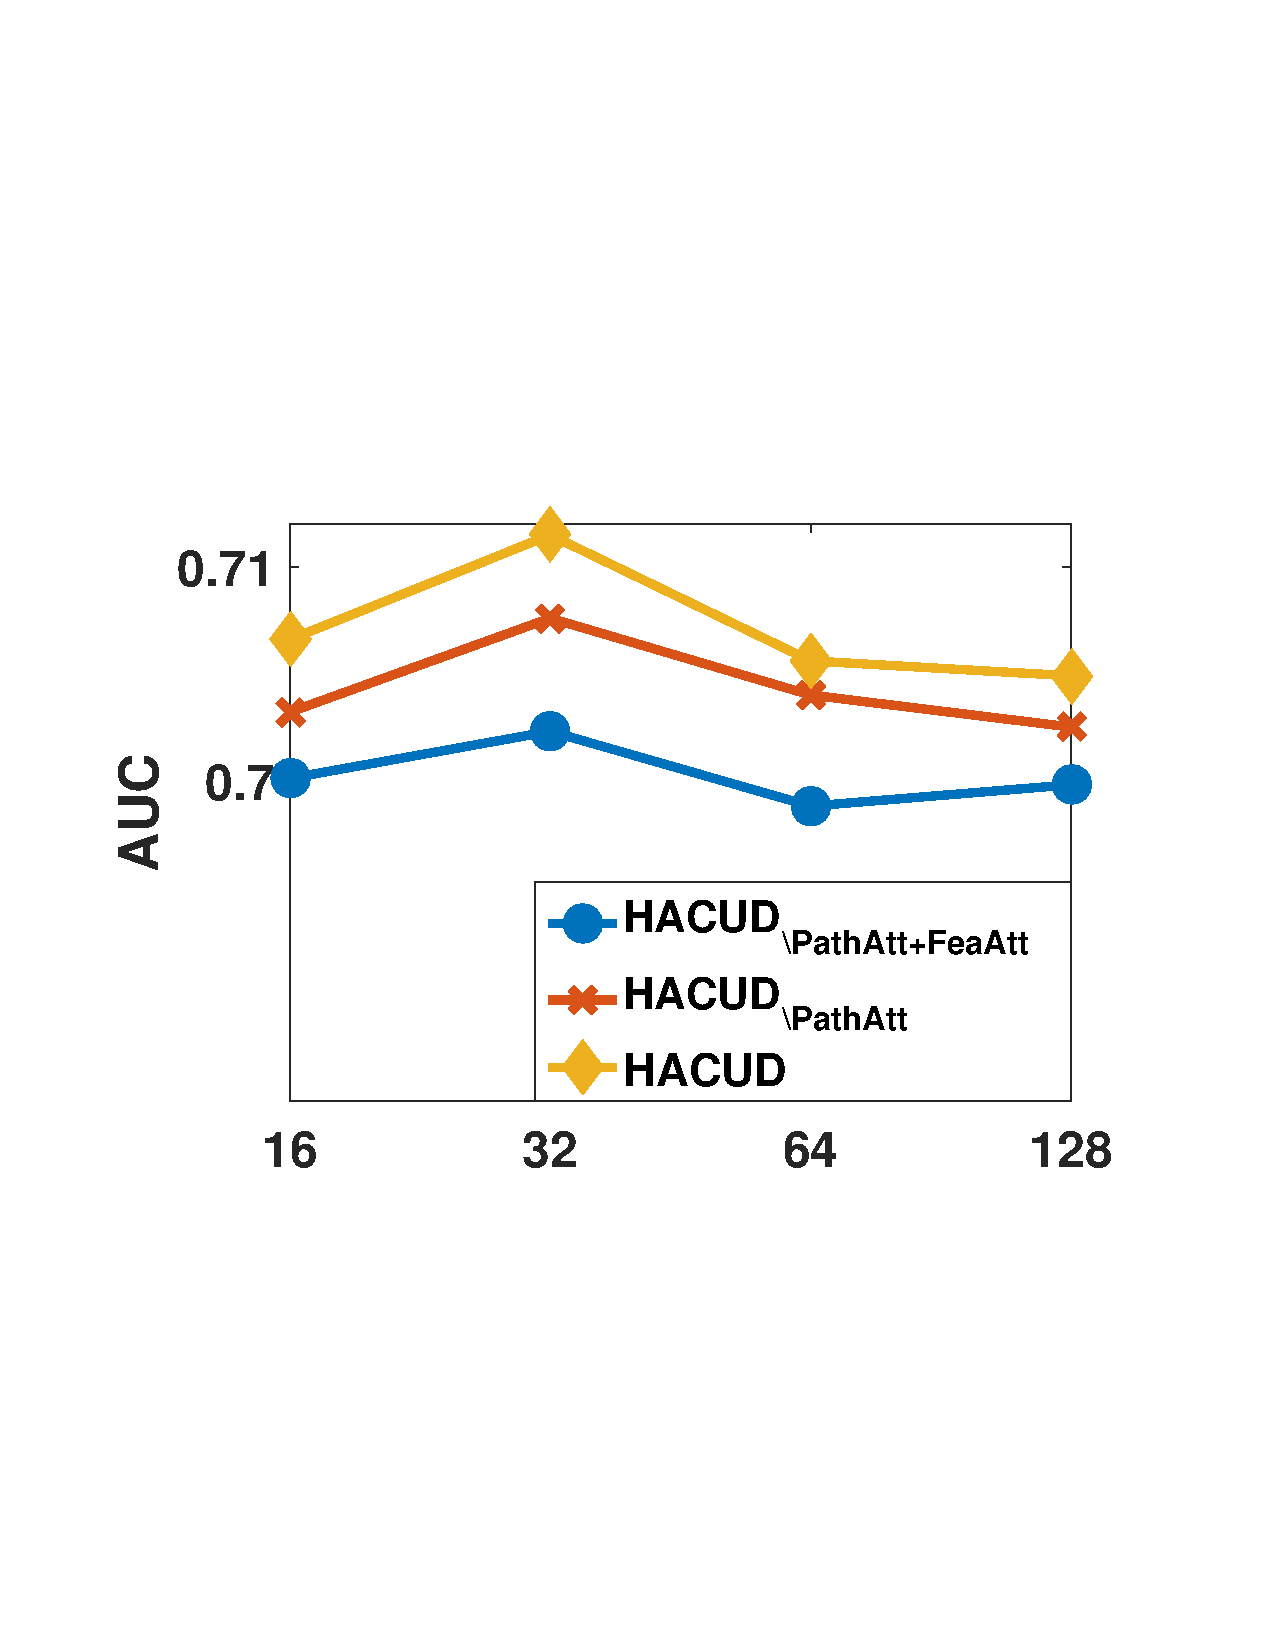
\includegraphics[width=4.0cm]{image/attention.pdf}
%\caption{Performance comparison of hierarchical attention \wrt the number of latent factors.}
%\label{fig-attention}
%\end{minipage}
%\begin{minipage}[t]{0.45\linewidth}
%\centering
%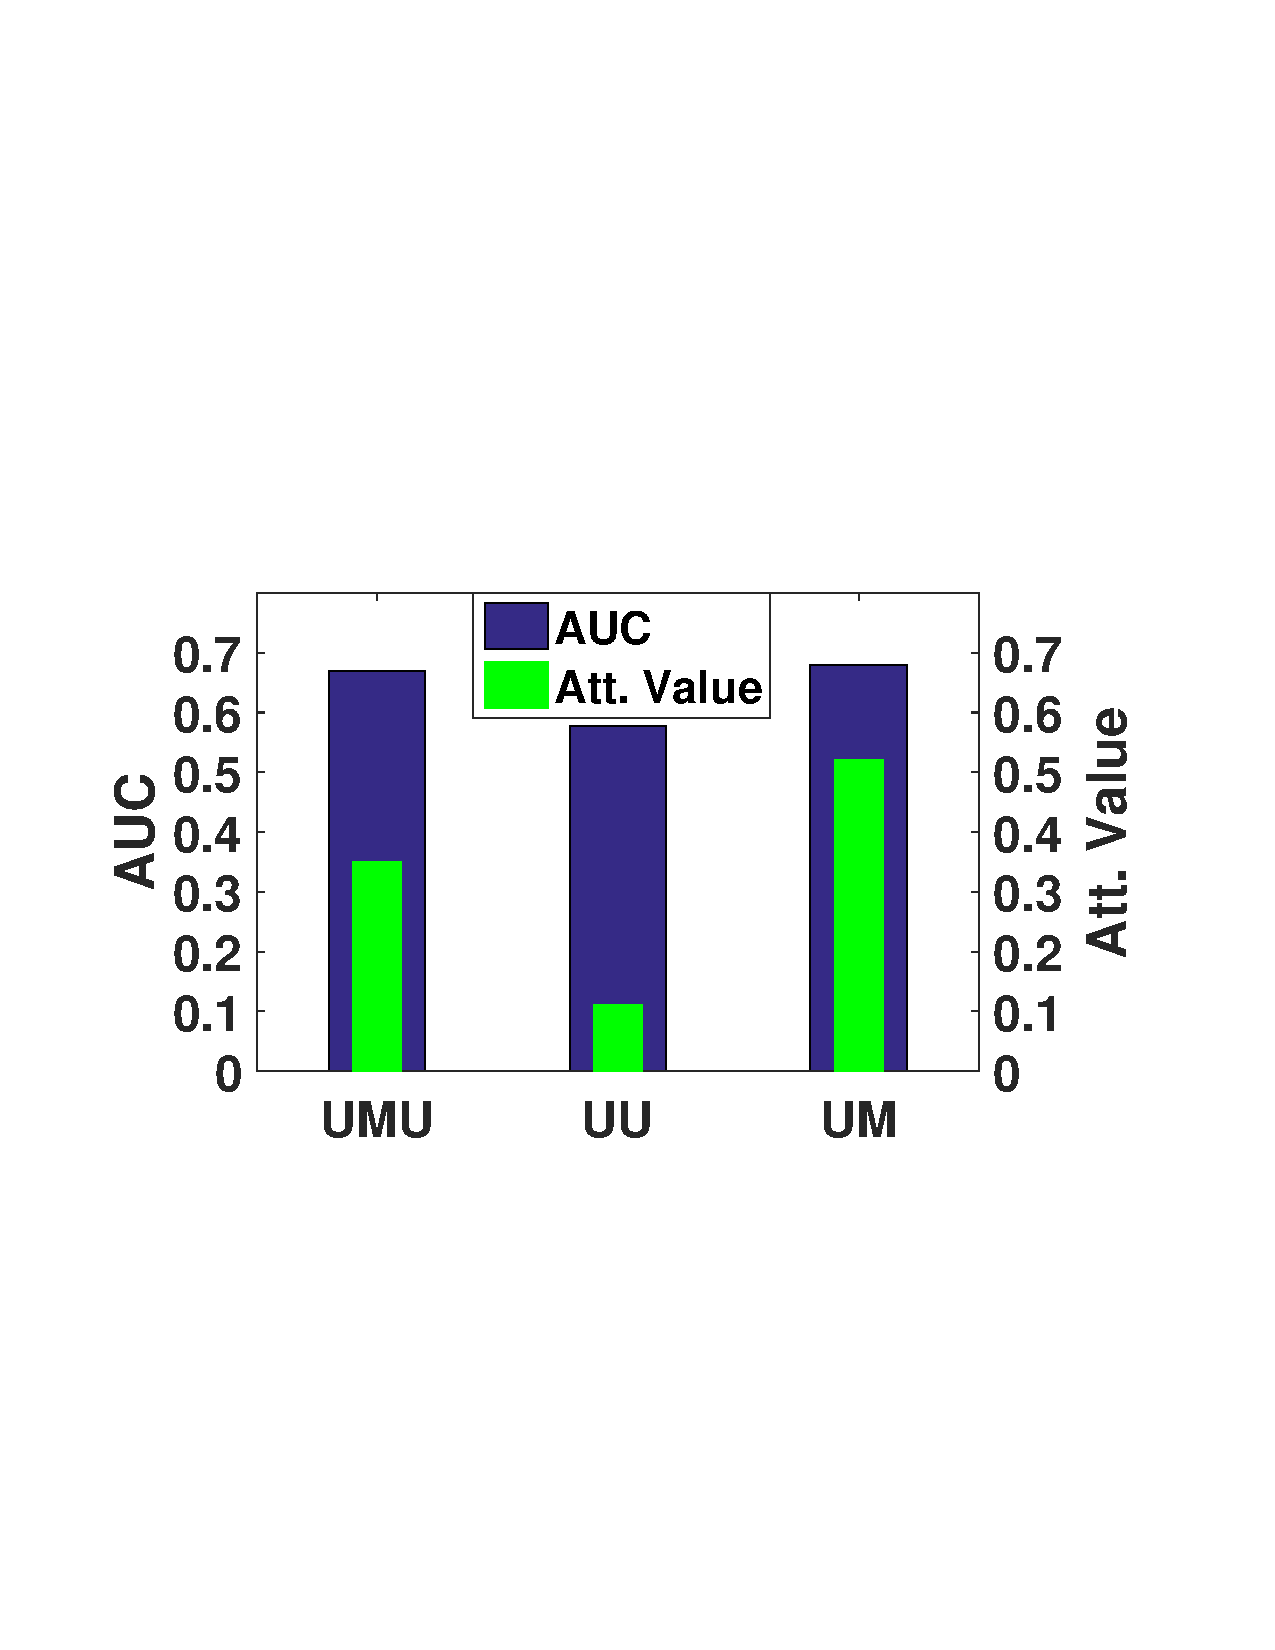
\includegraphics[width=4.6cm]{image/att_val.pdf}
%\caption{Comparison of performances on single meta-paths and the attention values of meta-paths.
%Meta-paths with better performances usually attract more attentions.
%}
%\label{fig-att_val}
%\end{minipage}
%\end{figure}

\begin{figure}[t]
\centering
\subfigure[Ten Days Dataset]{
\begin{minipage}[t]{0.45\linewidth}
\centering
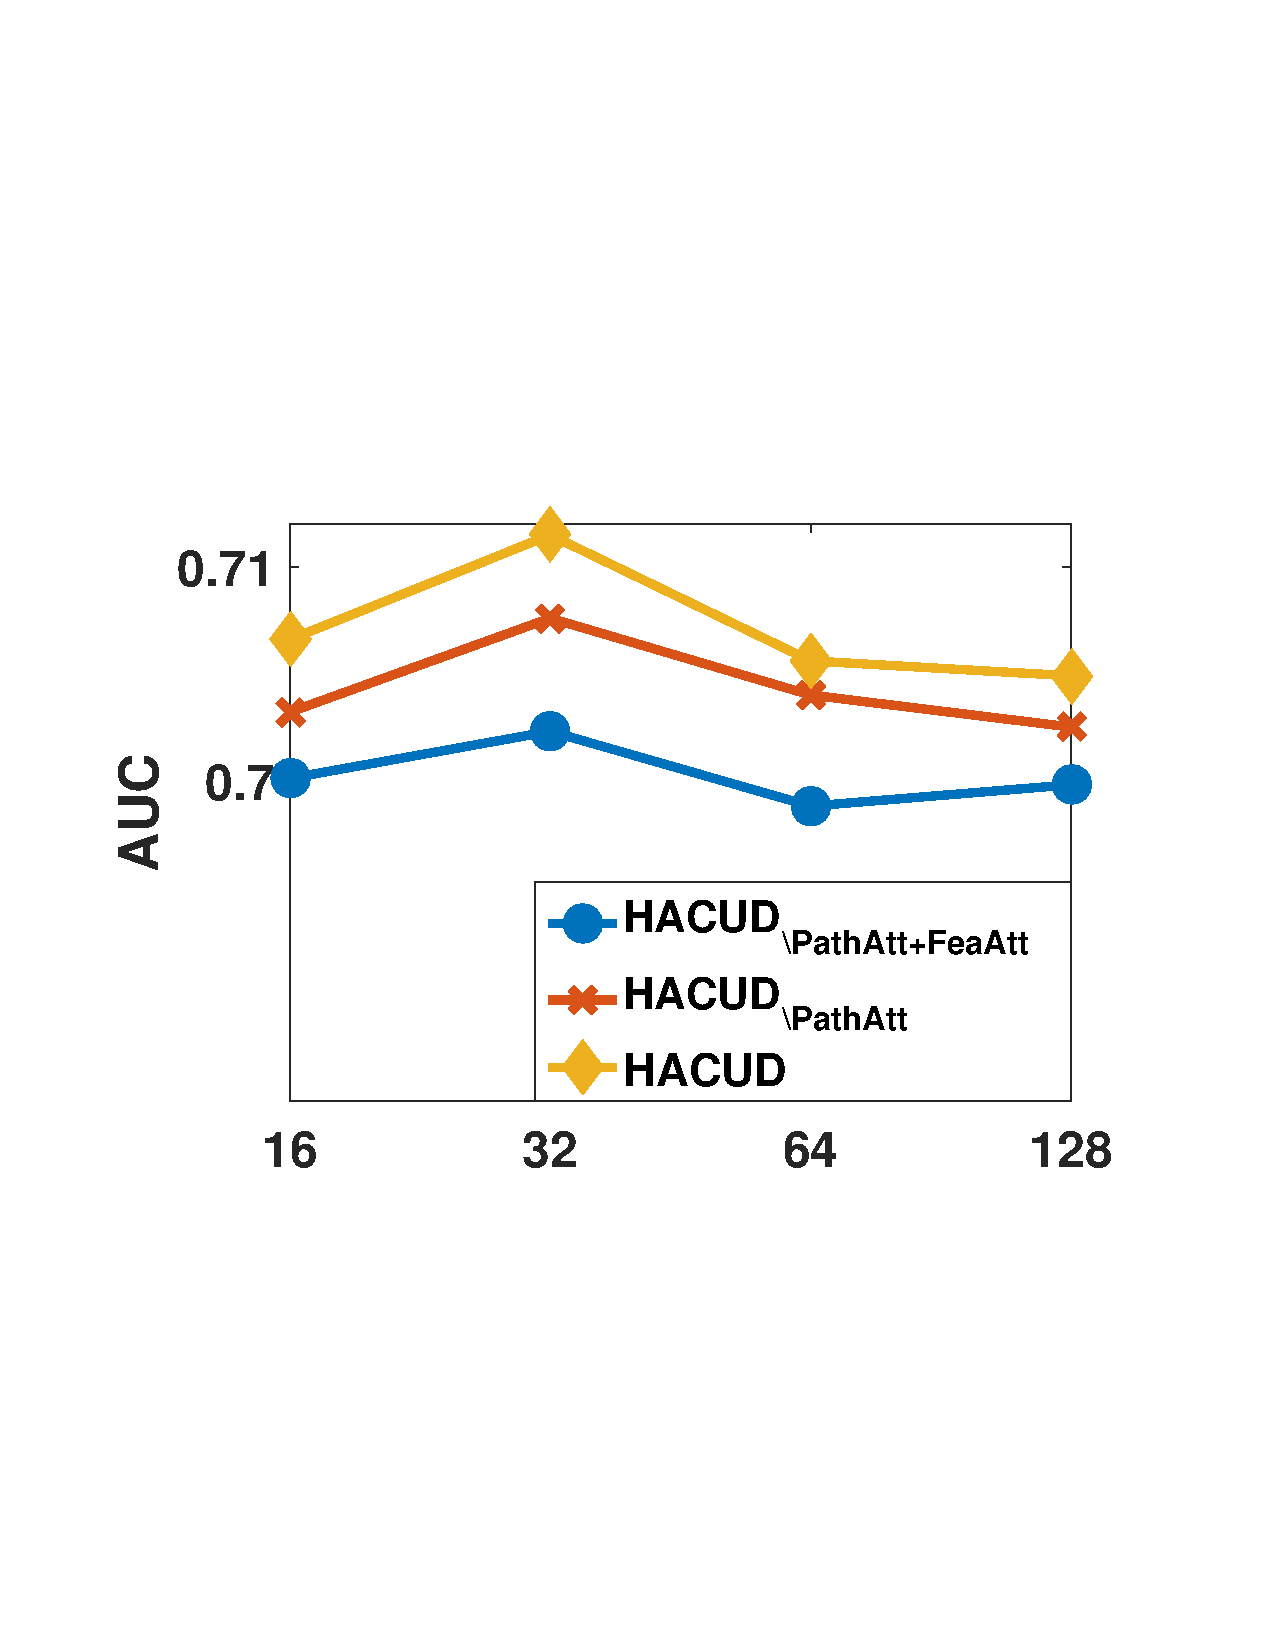
\includegraphics[width=4.1cm]{image/attention.pdf}
\end{minipage}
}
%\hspace{30pt}
\subfigure[One Month Dataset]{
\begin{minipage}[t]{0.45\linewidth}
\centering
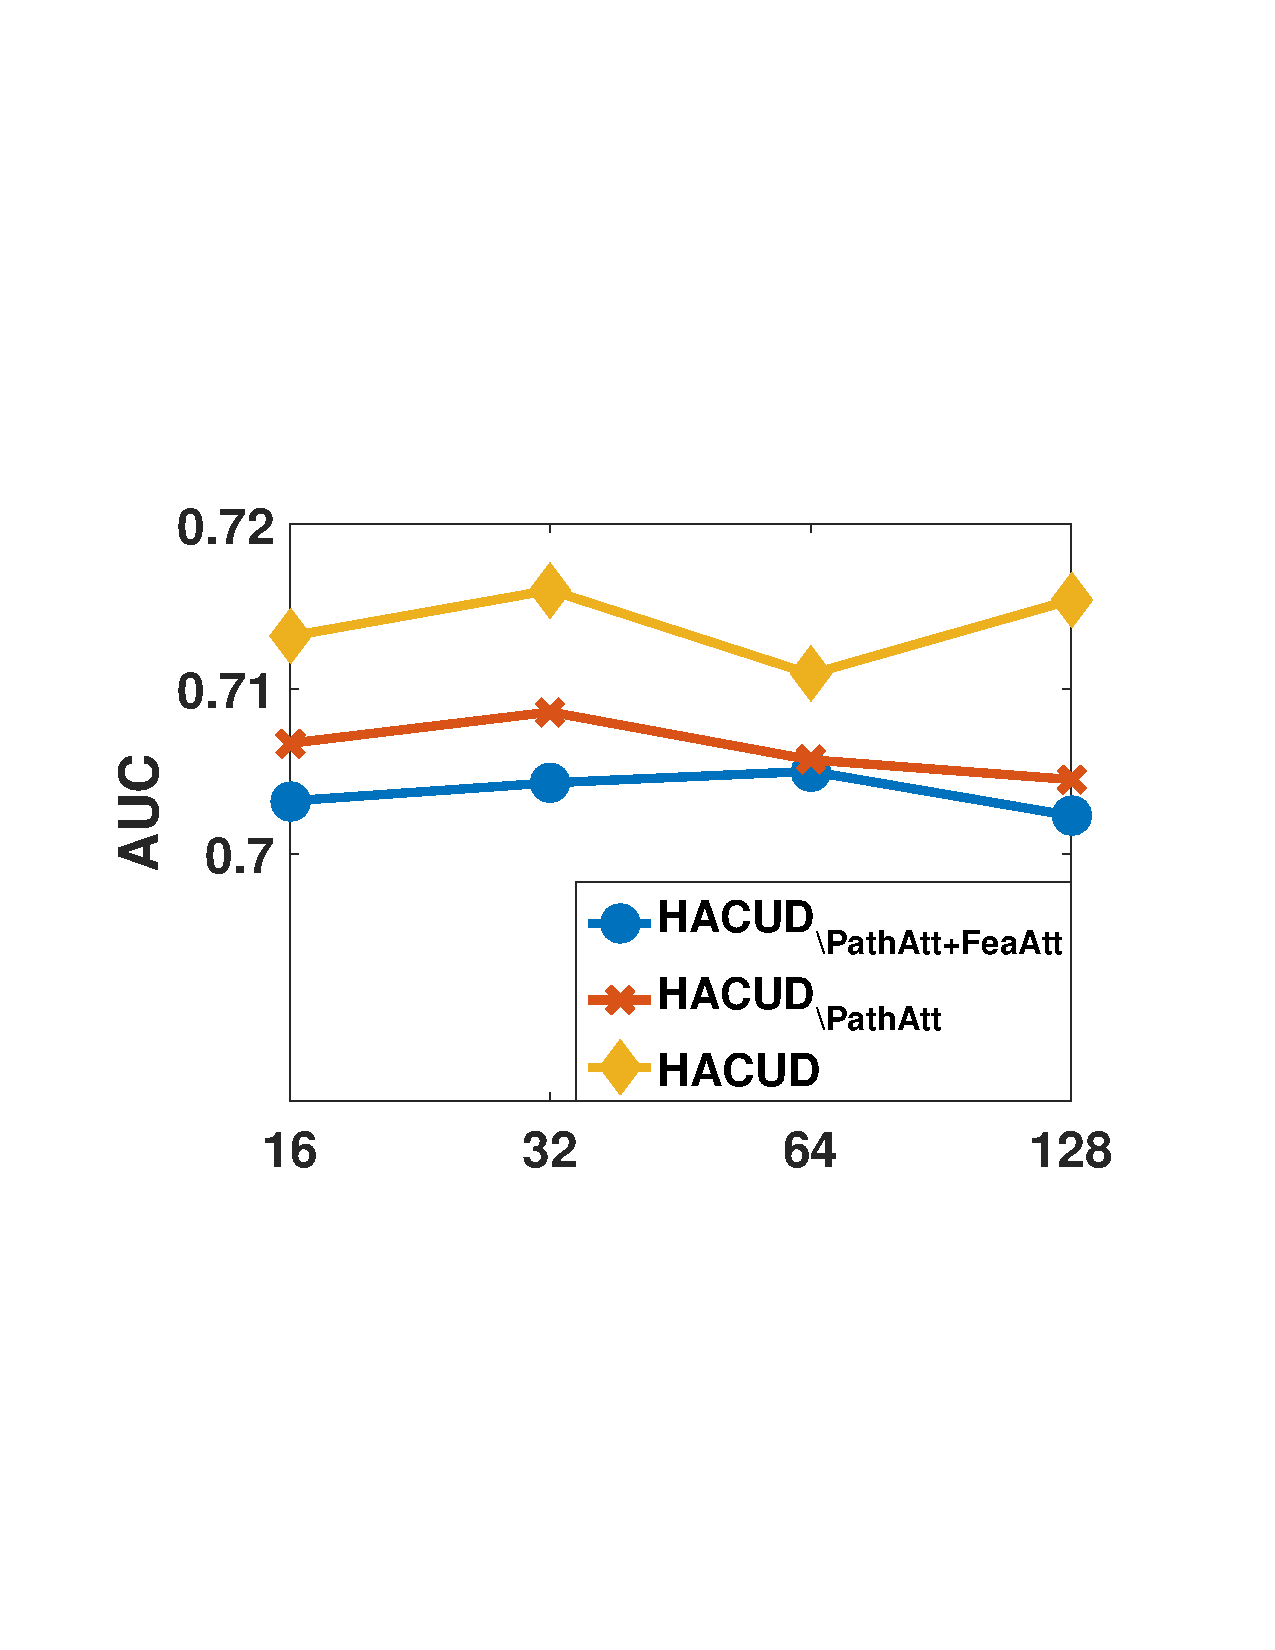
\includegraphics[width=4.1cm]{image/attention_large.pdf}
\end{minipage}
}
\caption{Performance comparison of hierarchical attention \wrt the dimension of latent representation $d$.\label{fig-attention}}
\end{figure}



\paratitle{Effects of Hierarchical Attention}. One of the major contributions of HACUD is hierarchical attention mechanism which learns the user preference towards features and meta-paths.
%is the incorporation of hierarchical attention mechanism, which takes the user's preference towards features and meta-paths into consideration for cash-out prediction. 
In order to examine its effectiveness, we compare our model with its two variants, namely HACUD$_{ \backslash PathAtt}$ (HACUD without path attention) and HACUD$_{\backslash PathAtt + FeaAtt}$ (HACUD without path and feature attention). 
For the performance comparison in Fig.~\ref{fig-attention}, 
%We report the performance comparison in the Fig.~\ref{fig-attention}. 
we can find that the overall performance order is as follows: HACUD $>$ HACUD$_{ \backslash PathAtt}$ $>$ HACUD$_{\backslash PathAtt + FeaAtt}$. The results show that the hierarchical mechanism is able to better utilize the user feature and features generated by meta-paths  in two aspects. First,  different meta-paths have different contributions to cash-out user prediction, which cannot be treated equally (\ie HACUD$_{ \backslash PathAtt}$). Second, each user tends to place different importance to the various attributes for each meta-path. Ignoring such influence may not be able to achieve the promising performance for fully exploiting attribute and structure information (\ie HACUD$_{\backslash PathAtt + FeaAtt}$).

Furthermore, we report the performances based on single meta path and corresponding average attention value in Fig.~\ref{fig-att_val}.  As we have observed, the performances of HACUD with different meta-paths and the corresponding attentions are positively correlated ( \ie important meta-paths tend to attract more attentions). In other words, the proposed HACUD model is potential to let different users focus on the proper meta-paths. %with the optimal performance, which reveal the effective of our path attention. %Obviously, the meta-path $UM$ and $UMU$ seem to be more important than others. One reasonable explanation is that cash-out users have aggregation effect.

\begin{figure}[t]
\centering
\subfigure[Ten Days Dataset]{
\begin{minipage}[t]{0.45\linewidth}
\centering
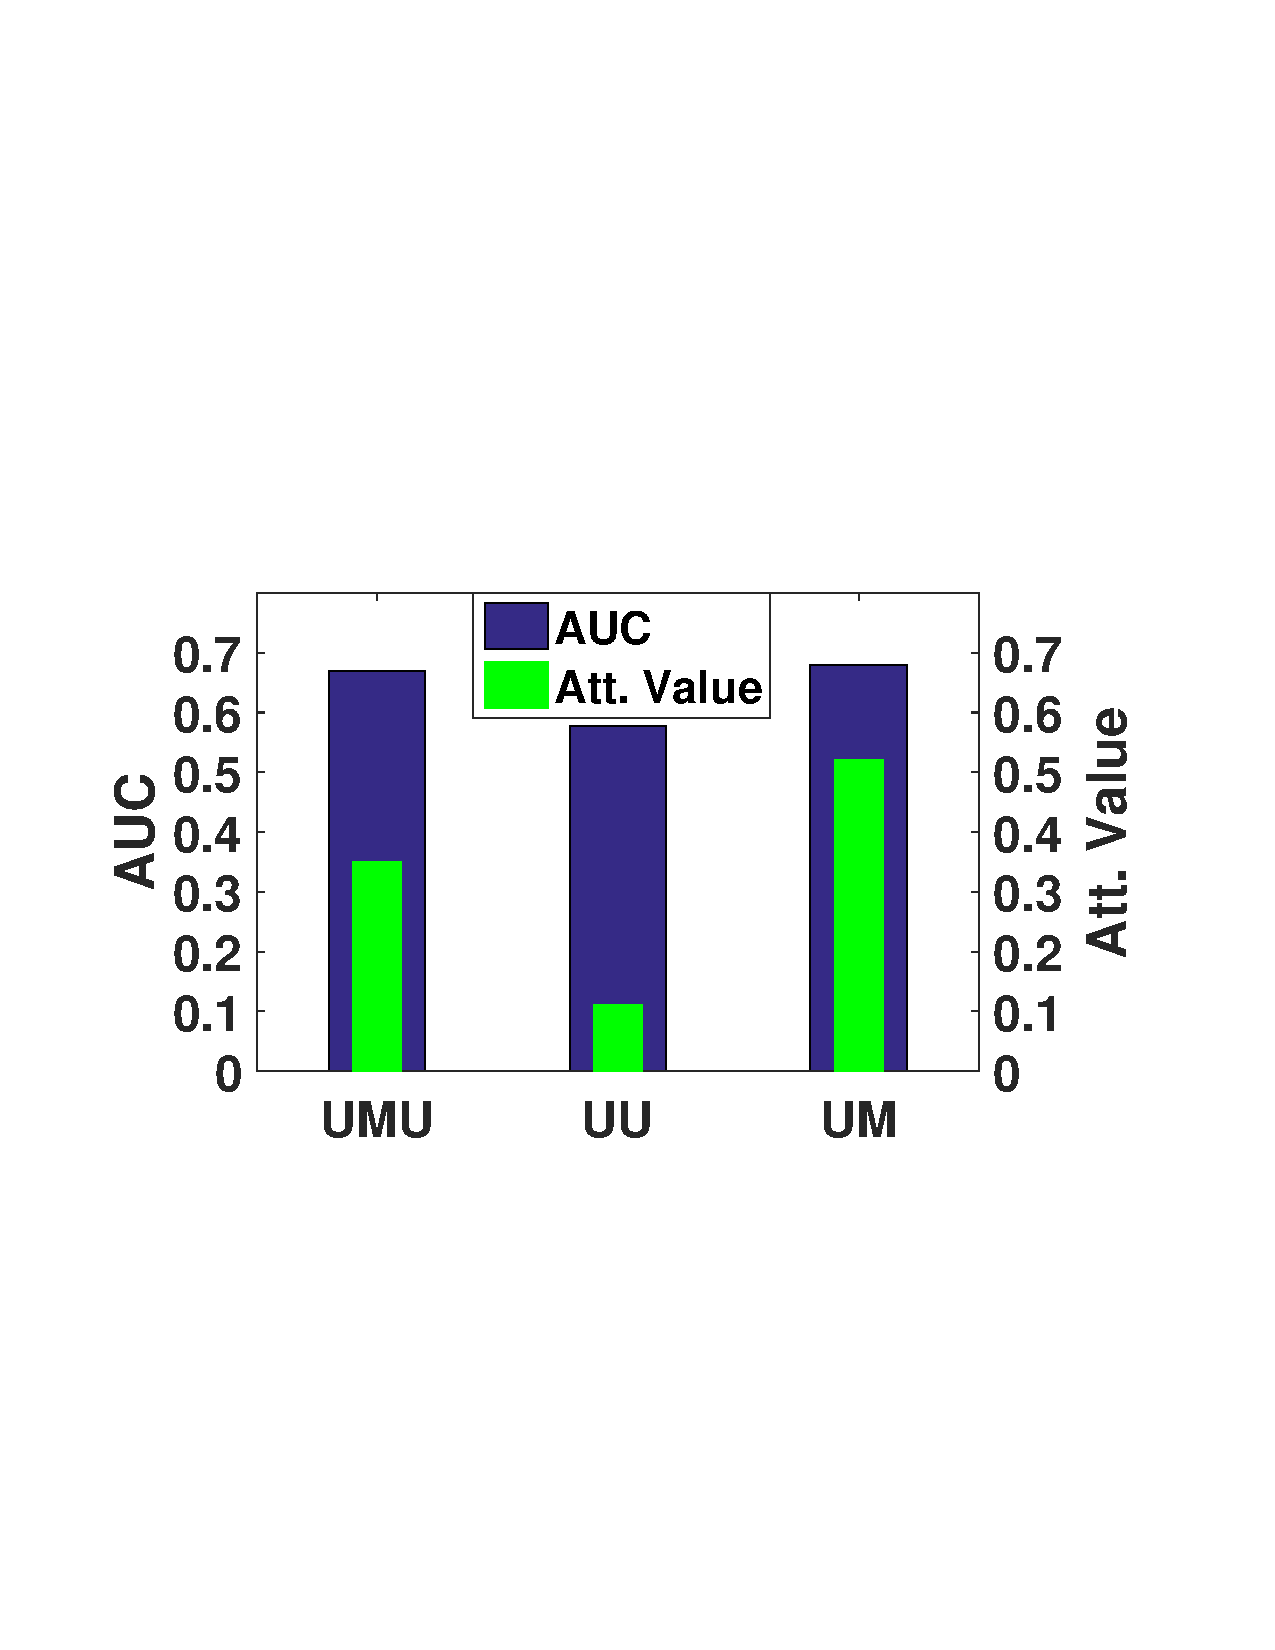
\includegraphics[width=4.2cm]{image/att_val.pdf}
\end{minipage}
}
%\hspace{30pt}
\subfigure[One Month Dataset]{
\begin{minipage}[t]{0.45\linewidth}
\centering
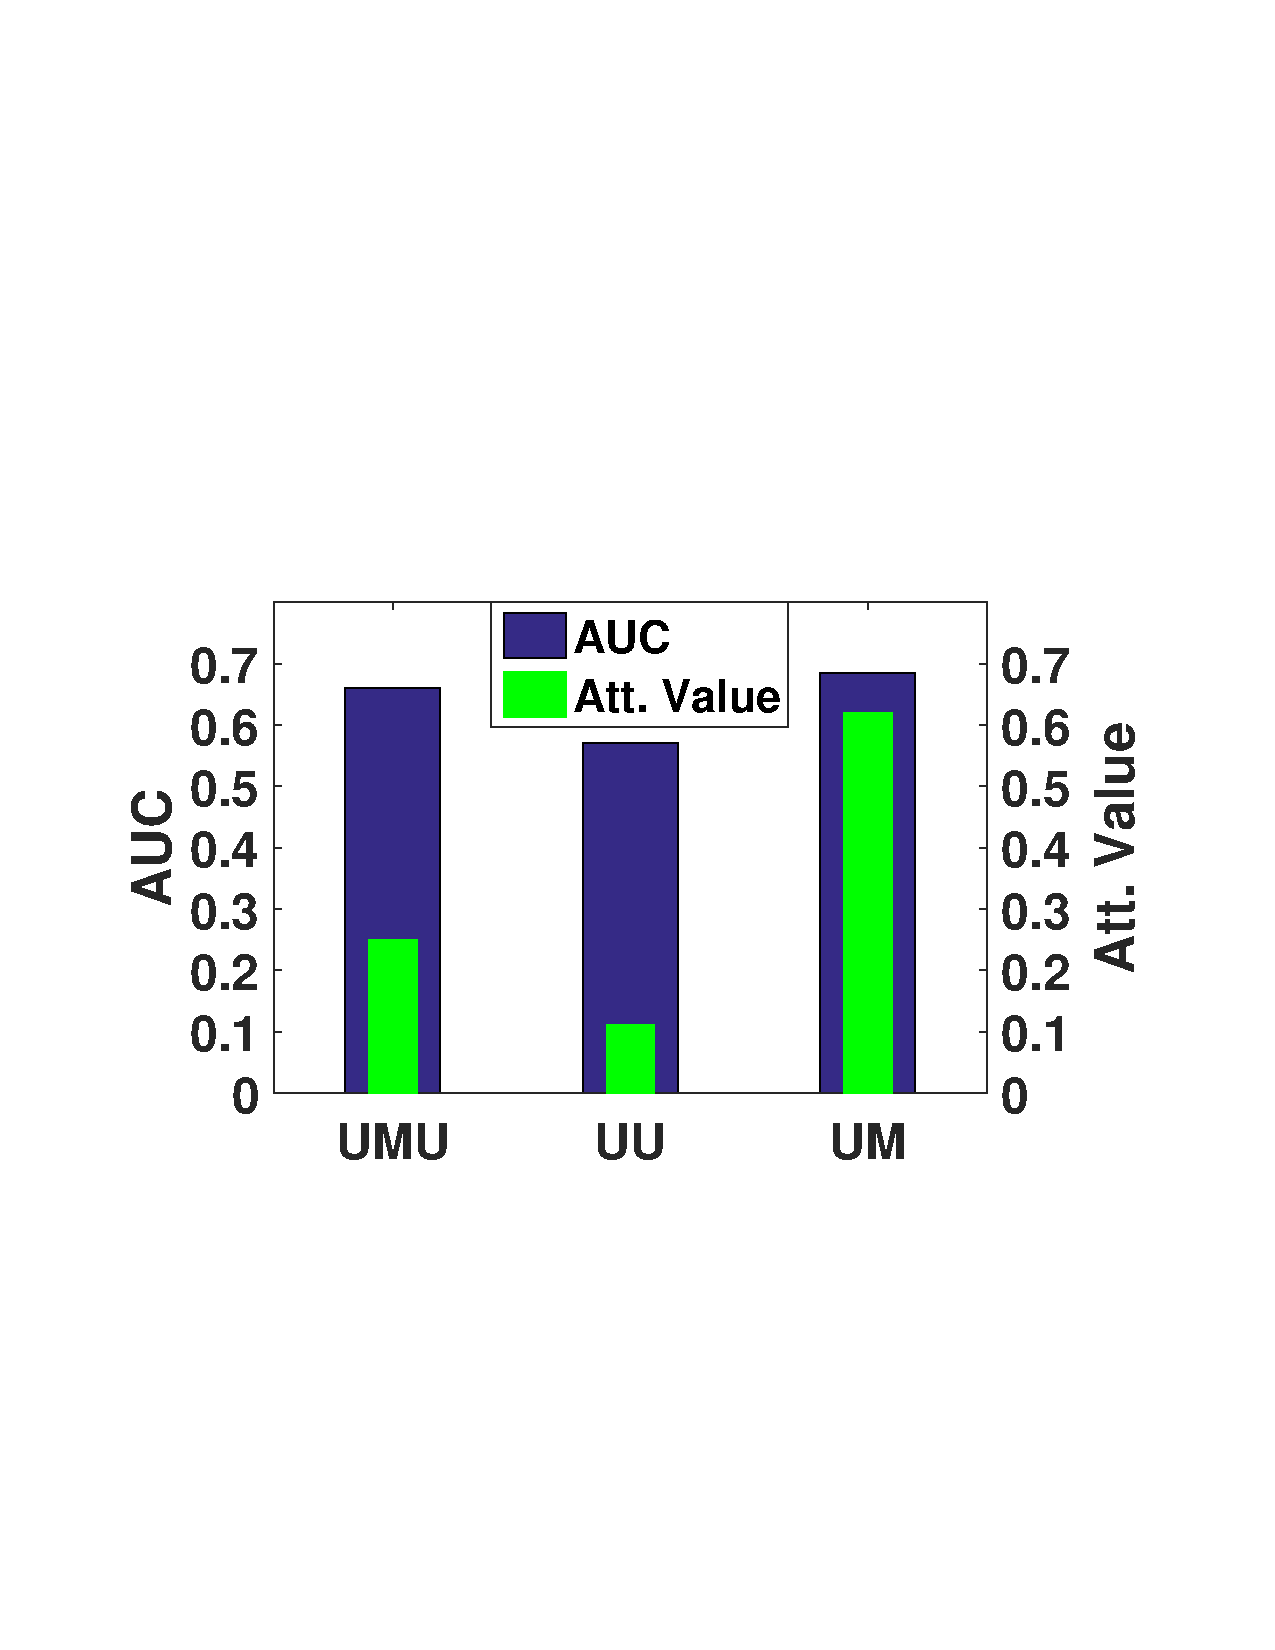
\includegraphics[width=4.0cm]{image/att_val_large.pdf}
\end{minipage}
}
\caption{Performances comparison on different meta-paths and corresponding attention values.\label{fig-att_val}}
\end{figure}
\paratitle{Impact of Different Meta-paths}.
As mentioned above, our model utilizes a selected set of meta-paths. To further analyze the impact of different meta-paths, we gradually incorporate  these meta-paths into our model and observe the performance change. In addition, we select GBDT as the baselines in this experiment. For convenience, we make the following denotation: (1) M$_1$ : user feature only; (2) M$_2$ : user feature + $UMU$; (3) M$_3$ : user feature + $UMU$ + $UU$; (3) M$_4$ : user feature + $UMU$ + $UU$ + $UM$.
As shown in the Fig.~\ref{fig-metapath}, we can observe that the performance would improve with the incorporation of more meta-paths, which demonstrates the effectiveness of structure information contained in different meta-paths. Specially, we can find that our model has a significant performance boost when adding the meta-paths $UMU$ and $UM$. This finding is consistent with previous observation in Fig.~\ref{fig-att_val}, where these two meta-paths have better performances, accompanying with higher attention values.


\paratitle{Parameter Tuning}
Besides the dimension of latent representation $d$ in Table~\ref{tab-eff}, our model also involves another important tuning parameter $\lambda$ in Eq.~\ref{equ-objective}.  We vary it in the set of  \{0.0, 0.0001, 0.001, 0.01, 0.1, 1.0\}. As shown in Fig. 5, the optimal performance is obtained near $\lambda = 0.01$, indicating that  $\lambda$ cannot be set too small or too large to prevent overfitting and underfitting.







\section{Related Work}
%In this section, we briefly review studies about heterogeneous information network and network embedding.

As a newly emerging direction, heterogeneous information network~\citep{shi2017survey} can model complex objects and their rich relations in real scenario. Due to the flexibility of HIN in modeling various kinds of heterogeneous data, many meta-path based search and mining tasks
have been explored in the past couple of years, including clustering~\citep{Sun2012Integrating}, classification~\citep{Ji2011Ranking} and recommendation~\citep{hu2018leveraging}. Considering the plentiful attributes in the nodes, \cite{Li2017Semi} further proposes attributed heterogeneous information network to enrich objects' information content and study the problem of clustering objects in an AHIN. Traditional network mining methods do not pay much attention to node attribute information, which may play important roles in real applications. Therefore, we firstly propose to model the cash-out users detection problem as a classification problem in AHIN.

\begin{figure}[t]
\begin{minipage}[t]{0.45\linewidth}
\centering
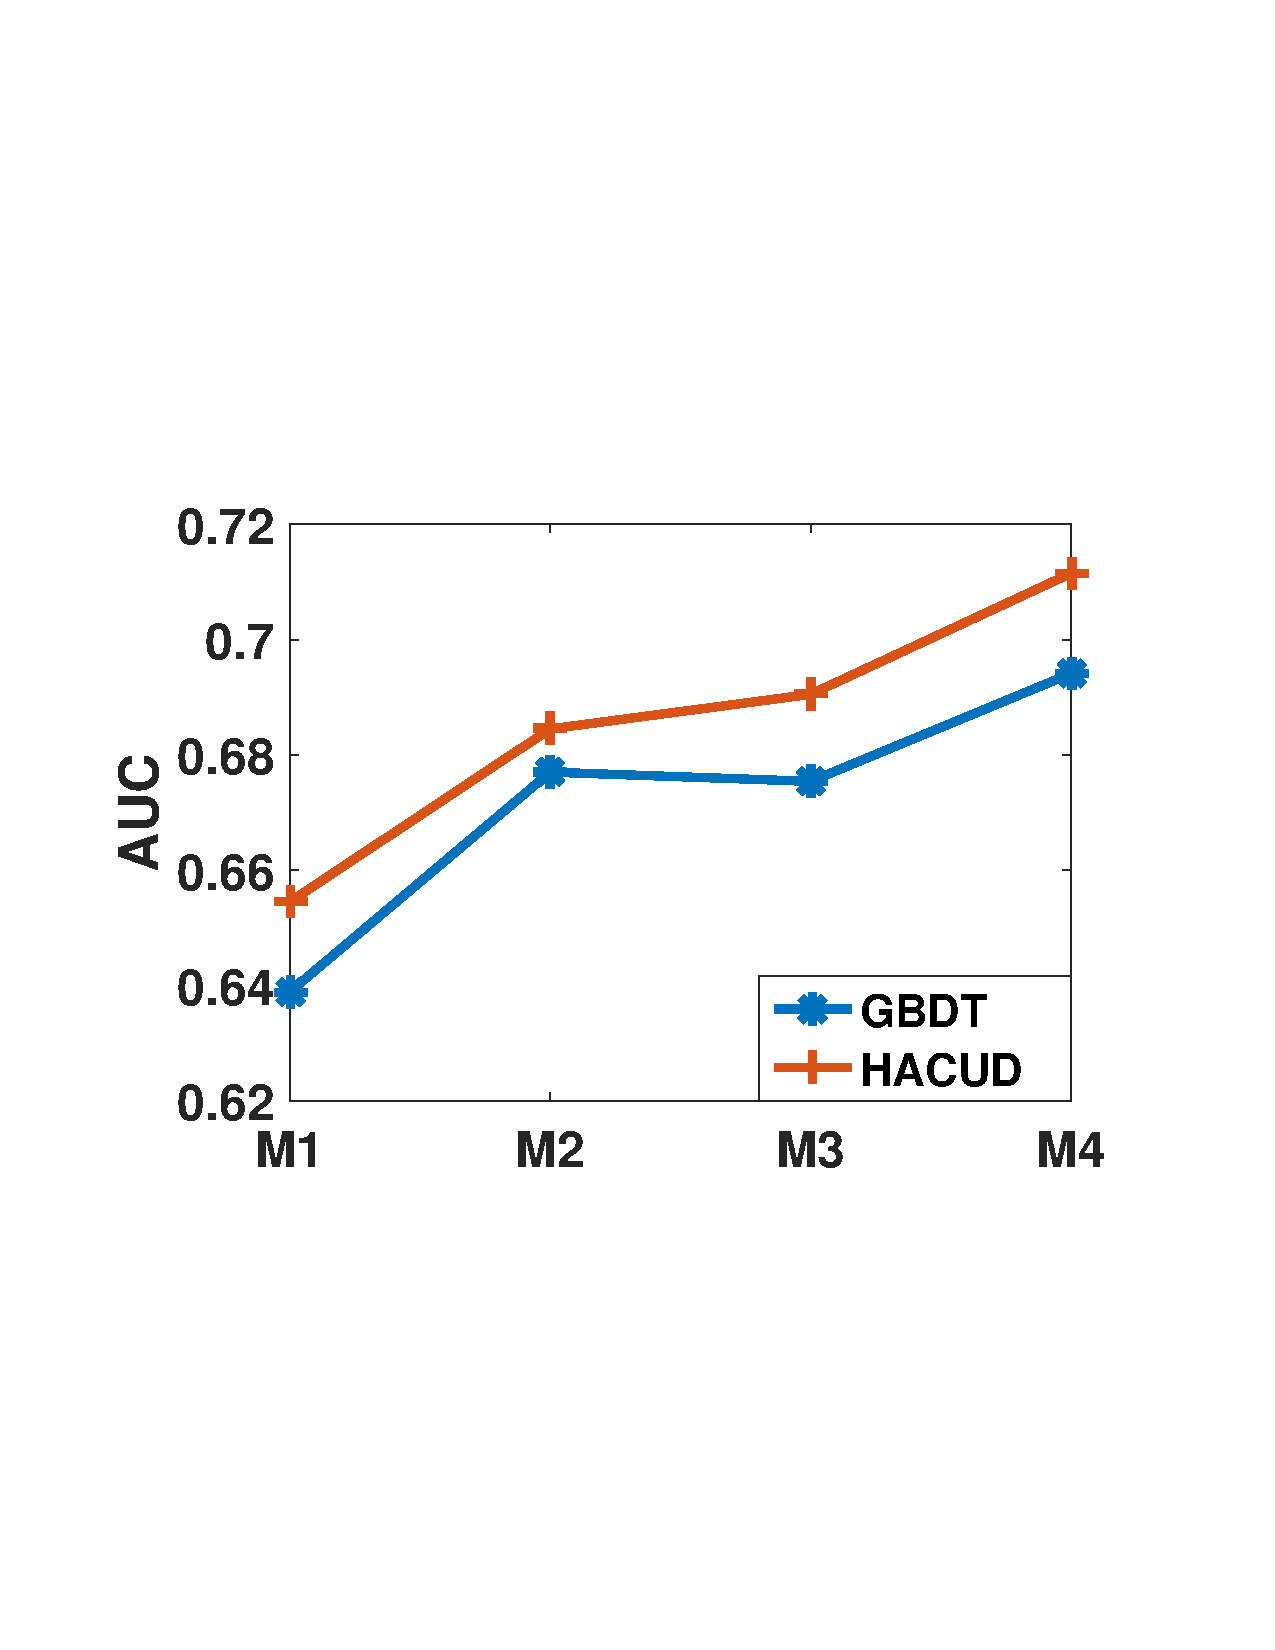
\includegraphics[width=4.1cm]{image/metapath.pdf}
\caption{Impact of different meta-paths on Ten Days Dataset.}
\label{fig-metapath}
\end{minipage}
\begin{minipage}[t]{0.45\linewidth}
\centering
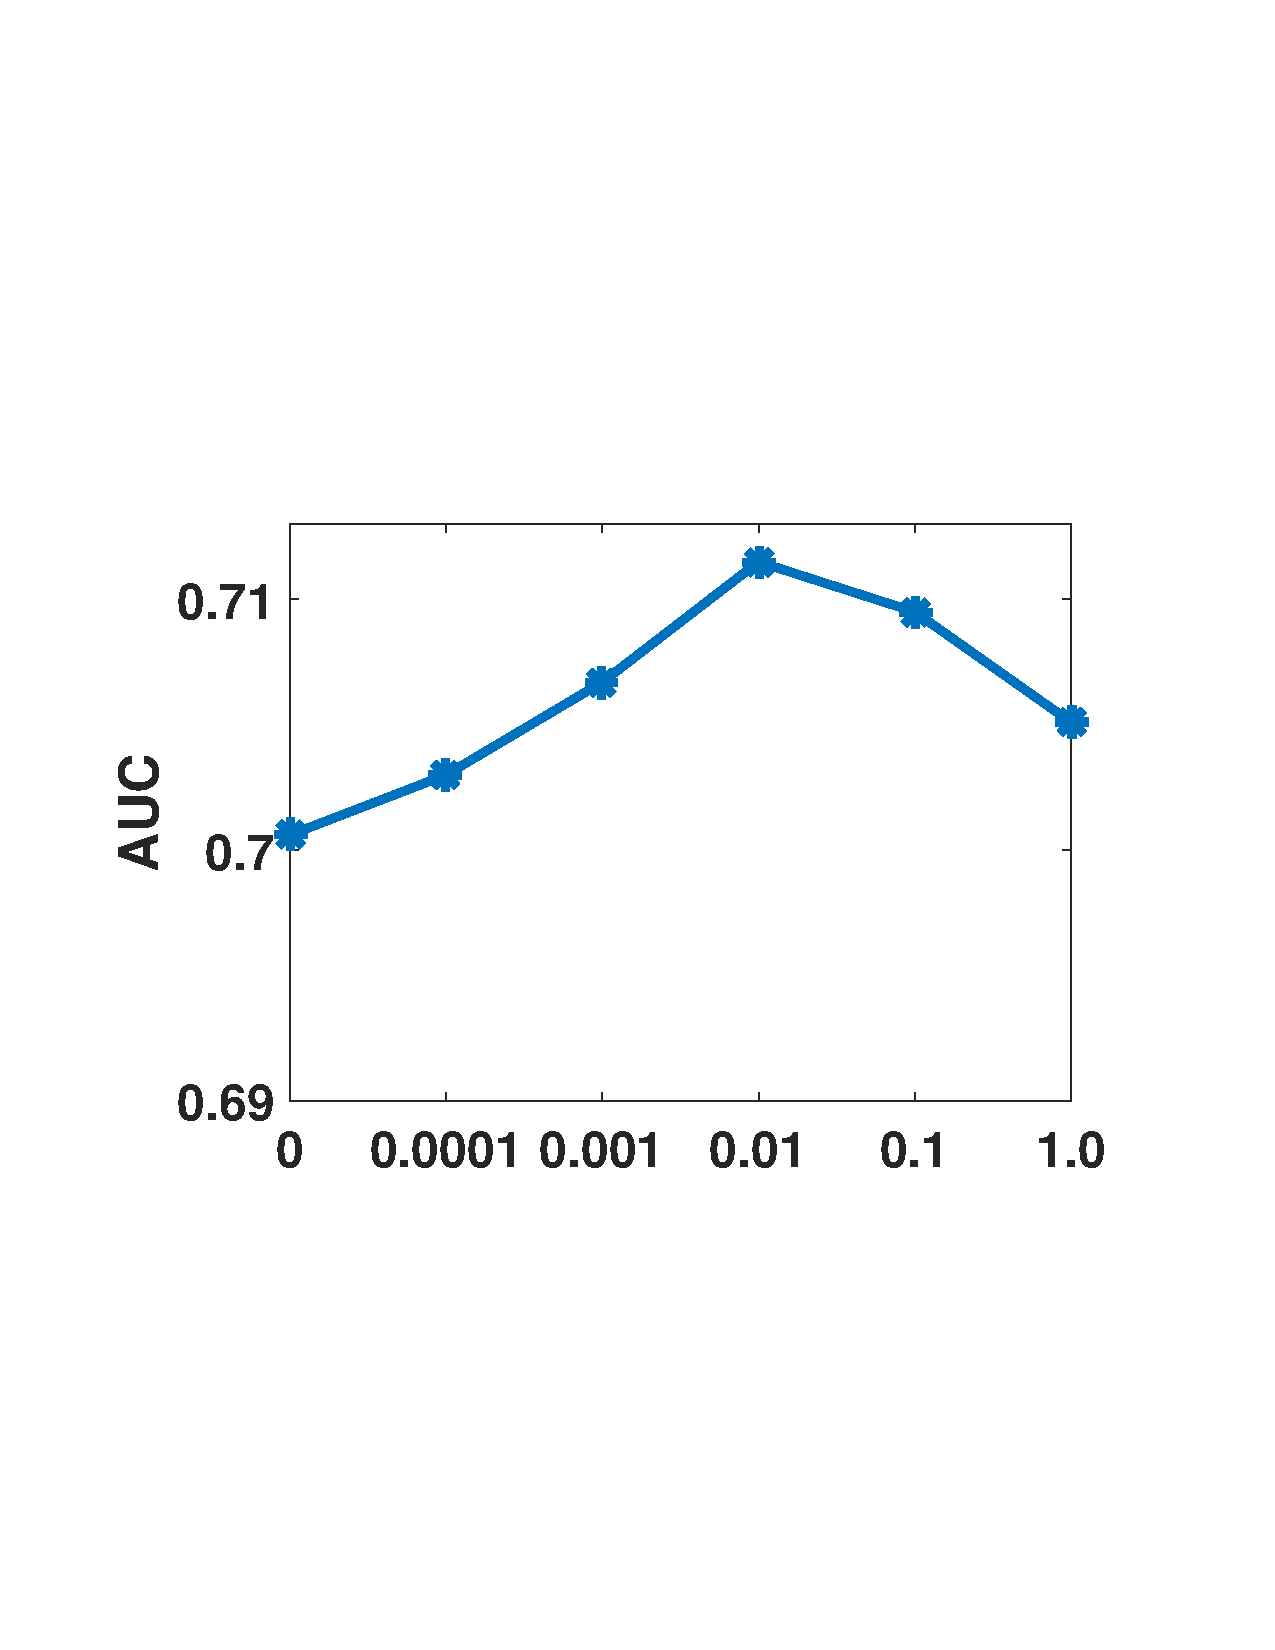
\includegraphics[width=4.1cm]{image/lambda.pdf}
\caption{Impact of parameter $\lambda$  on Ten Days Dataset.}
\label{fig-lambda}
\end{minipage}
\end{figure}

On the other hand, network embedding has shown its potential in structure feature extraction and has been successfully applied in many data mining tasks. Early network embedding methods focus on homogeneous network, which usually utilize network context information to represent nodes, \eg random walk based context~\citep{Perozzi2014DeepWalk,grover2016node2vec}, network neighborhood~\citep{wang2016structural,Tang2015LINE}, high order network proximity~\citep{Cao2015GraRep}. Recently, attention is increasingly shifting towards heterogeneous network.  \cite{dong2017metapath2vec} obtain the context of nodes with meta-path based random walk and learn the HIN embedding through heterogeneous skip-gram model, while \cite{Fu2017HIN2Vec} capture rich relation semantics via neural network. Moreover, there are also several works attempting to fully analyze networks via embedding methods with features and labeled data, including GCN~\citep{Kipf2016Semi}, Structure2vec~\citep{dai2016discriminative} and so on. Unfortunately, these methods are usually designed for specific task and only exploit partial information in networks, therefore they cannot be directly applied in the AHIN and the cash-out user detection problem for promising performance.
\section{Conclusion}
%In this paper, we firstly study the cash-out user detection problem from network structure perspective and propose a novel HACUD model for the purpose. To characterize the complex and heterogeneous cash-out fraud scene, we model the plentiful attributes of users and rich relations between users as an attributed heterogeneous information network. Next, we design a hierarchical attention mechanism to model user's preferences towards attribute information and meta-paths. Finally, with the real datasets in Ant Credit Pay of Ant Financial Services Group, we do extensive experiments for the cash-user detection problem, and demonstrate the effectiveness of the proposed model compared to the state of arts. As future work, we will investigate to integrating more heterogeneous information (\ie more relative objects and interaction relations between them) and extending our model to semi-supervised scene.

In this paper, we first study the cash-out user detection problem under the attributed heterogenous information network
framework, constituted by objects and their relations in the scenario of credit payment service, and propose a novel HACUD model
for the purpose. With the help of meta-path based neighbors, we aggregate features of objects  from node attributes,
as well as structure features generated by meta-paths. Furthermore, we design a hierarchical attention mechanism to
model user preferences towards attributes and meta-paths. With the real datasets in Ant Credit Pay of Ant Financial Services Group, extensive experiments for the cash-user detection  task demonstrate the effectiveness of our model. As future work, we will investigate to integrating more heterogeneous information (\eg interaction relations) and extending our model to semi-supervised scenario.

%As future work, we will investigate to 
%integrating more heterogeneous information and 
%extending our model to semi-supervised scene.
\section{Acknowledgement}
We would like to thank Feng Zhao, Yanming Fang and Quan Yu, from the Risk Management Department of MYbank in Ant Financial Service Group. This work is supported in part by the National Natural Science Foundation of China (No. 61772082, 61702296, 61806020,61375058), the National Key Research and Development Program of China (2017YFB0803304) and the Beijing Municipal Natural Science Foundation (4182043).

%\clearpage
\bibliography{references}
\bibliographystyle{aaai}



\end{document}
